%===============================================================================
% LaTeX sjabloon voor de bachelorproef toegepaste informatica aan HOGENT
% Meer info op https://github.com/HoGentTIN/latex-hogent-report
%===============================================================================

\documentclass[dutch,dit,thesis]{hogentreport}

% TODO:
% - If necessary, replace the option `dit`' with your own department!
%   Valid entries are dbo, dbt, dgz, dit, dlo, dog, dsa, soa
% - If you write your thesis in English (remark: only possible after getting
%   explicit approval!), remove the option "dutch," or replace with "english".

\usepackage{lipsum} % For blind text, can be removed after adding actual content

%% Pictures to include in the text can be put in the graphics/ folder
\graphicspath{{graphics/}}

%% For source code highlighting, requires pygments to be installed
%% Compile with the -shell-escape flag!
\usepackage[section]{minted}
\usemintedstyle{solarized-light}
\definecolor{bg}{RGB}{253,246,227} %% Set the background color of the codeframe

%% Change this line to edit the line numbering style:
\renewcommand{\theFancyVerbLine}{\ttfamily\scriptsize\arabic{FancyVerbLine}}

%% Macro definition to load external java source files with \javacode{filename}:
\newmintedfile[javacode]{java}{
    bgcolor=bg,
    fontfamily=tt,
    linenos=true,
    numberblanklines=true,
    numbersep=5pt,
    gobble=0,
    framesep=2mm,
    funcnamehighlighting=true,
    tabsize=4,
    obeytabs=false,
    breaklines=true,
    mathescape=false
    samepage=false,
    showspaces=false,
    showtabs =false,
    texcl=false,
}

% Other packages not already included can be imported here
\usepackage{xcolor}
\usepackage{listings}


% Define Dockerfile listing style
\lstdefinestyle{dockerfile}{
  basicstyle=\footnotesize\ttfamily\color{black},
  backgroundcolor=\color{gray!5},
  keywordstyle=\color{blue},
  keywords={FROM, RUN, COPY, ADD, ENV, WORKDIR, EXPOSE},
  breaklines=true,
  prebreak=\raisebox{0ex}[0ex][0ex]{\ensuremath{\hookleftarrow}},
  tabsize=2,
  showstringspaces=false,
  commentstyle=\color{green!70!black},
  stringstyle=\color{orange},
  captionpos=b,
  framesep=10pt,
  xleftmargin=15pt,
  framexleftmargin=5pt,
  framexrightmargin=5pt,
  framextopmargin=5pt,
  framexbottommargin=5pt
}

% Define Dockerfile language for lstlisting
\lstdefinelanguage{Dockerfile}{
  morekeywords={FROM, RUN, COPY, ADD, ENV, WORKDIR, EXPOSE},
  morecomment=[l]{\#},
  commentstyle=\color{green!70!black},
  morestring=[b]",
  stringstyle=\color{orange}
}

\lstset{
  language=Java,
  basicstyle=\footnotesize\ttfamily\color{black},
  backgroundcolor=\color{gray!5},
  keywordstyle=\color{blue},
  keywords={public, class, static, void, main, String},
  breaklines=true,
  prebreak=\raisebox{0ex}[0ex][0ex]{\ensuremath{\hookleftarrow}},
  tabsize=2,
  showstringspaces=false,
  commentstyle=\color{gray},
  stringstyle=\color{green!50!black},
  captionpos=b,
  framesep=10pt,
  xleftmargin=15pt,
  framexleftmargin=5pt,
  framexrightmargin=5pt,
  framextopmargin=5pt,
  framexbottommargin=5pt
}

\lstdefinestyle{mystyle}{
    backgroundcolor=\color{gray!5},
    basicstyle=\footnotesize\ttfamily\color{black},
    commentstyle=\color{gray},
    keywordstyle=\color{blue},
    stringstyle=\color{orange},
    identifierstyle=\color{purple},
    showstringspaces=false,
    breaklines=true,
    numbers=left,
    numberstyle=\tiny\color{gray},
    language=Java,
    captionpos=b,
    frame=single,
    framerule=0pt,
    framesep=10pt,
    xleftmargin=15pt,
    framexleftmargin=5pt,
    framexrightmargin=5pt,
    framextopmargin=5pt,
    framexbottommargin=5pt,
    tabsize=4,
    morekeywords={public, class, static, void},
    keywordstyle=\color{blue},
    morekeywords=[2]{App},
    keywordstyle=[2]\color{green!50!black},
    morestring=[b]",
    stringstyle=\color{orange},
    morecomment=[l]{//},
    commentstyle=\color{green!50!black}
}

% Define Kubernetes YAML listing style
\lstdefinestyle{kubernetesyaml}{
  basicstyle=\footnotesize\ttfamily\color{black},
  backgroundcolor=\color{gray!5},
  keywordstyle=\color{blue},
  keywords={apiVersion, kind, metadata, spec, containers, name, image, port, protocol},
  stringstyle=\color{orange},
  commentstyle=\color{green},
  captionpos=b,
  framesep=10pt,
  xleftmargin=15pt,
  framexleftmargin=5pt,
  framexrightmargin=5pt,
  framextopmargin=5pt,
  framexbottommargin=5pt
}

% Define Kubernetes YAML language for lstlisting
\lstdefinelanguage{kubernetesyaml}{
  keywords={apiVersion, kind, metadata, spec, containers, name, image, port, protocol},
  sensitive=false,
  comment=[l]{\#},
  morestring=[b]',
  morestring=[b]",
  moredelim=[s][\color{blue}\ttfamily]{:}{\ },
  moredelim=[s][\color{orange}\ttfamily]{=}{\ },
  moredelim=[l][\color{green}]{\#}
}

\definecolor{codegreen}{RGB}{60,128,49}
\definecolor{codeorange}{RGB}{204,96,0}
\definecolor{codeblue}{RGB}{0,96,204}
\definecolor{codeskyblue}{RGB}{51,153,204}
\definecolor{codepurple}{RGB}{128,0,128}

\lstdefinelanguage{terraform}{
    morekeywords=[1]{resource,data,locals,module,provider,variable,output,terraform},
    keywordstyle=[1]\color{codegreen},
    morekeywords=[2]{count,for_each,if,else},
    keywordstyle=[2]\color{codeblue},
    morekeywords=[3]{true,false},
    keywordstyle=[3]\color{codepurple},
    morestring=[b]",
    stringstyle=\color{black},
    comment=[l]{\#},
    commentstyle=\color{codeorange}\ttfamily,
    identifierstyle=\color{codeskyblue},
    sensitive=true,
    keepspaces=true,
    breaklines=true,
    tabsize=2,
}

\usepackage{dirtree}

%%---------- Document metadata -------------------------------------------------
% TODO: Replace this with your own information
\author{Victor Vanhooren}
\supervisor{Dhr. F. Van Houte}
\cosupervisor{Mevr. S. Beeckman}
\title[Optionele ondertitel]%
    {Titel van de bachelorproef}
\academicyear{\advance\year by -1 \the\year--\advance\year by 1 \the\year}
\examperiod{1}
\degreesought{\IfLanguageName{dutch}{Professionele bachelor in de toegepaste informatica}{Bachelor of applied computer science}}
\partialthesis{false} %% To display 'in partial fulfilment'
%\institution{Internshipcompany BVBA.}

%% Add global exceptions to the hyphenation here
\hyphenation{back-slash}

%% The bibliography (style and settings are  found in hogentthesis.cls)
\addbibresource{bachproef.bib}            %% Bibliography file
\addbibresource{../voorstel/voorstel.bib} %% Bibliography research proposal
\defbibheading{bibempty}{}

%% Prevent empty pages for right-handed chapter starts in twoside mode
\renewcommand{\cleardoublepage}{\clearpage}

\renewcommand{\arraystretch}{1.2}

%% Content starts here.
\begin{document}

%---------- Front matter -------------------------------------------------------

\frontmatter

\hypersetup{pageanchor=false} %% Disable page numbering references
%% Render a Dutch outer title page if the main language is English
\IfLanguageName{english}{%
    %% If necessary, information can be changed here
    \degreesought{Professionele Bachelor toegepaste informatica}%
    \begin{otherlanguage}{dutch}%
       \maketitle%
    \end{otherlanguage}%
}{}

%% Generates title page content
\maketitle
\hypersetup{pageanchor=true}

%%=============================================================================
%% Voorwoord
%%=============================================================================

\chapter*{\IfLanguageName{dutch}{Woord vooraf}{Preface}}%
\label{ch:voorwoord}

%% TODO:
%% Het voorwoord is het enige deel van de bachelorproef waar je vanuit je
%% eigen standpunt (``ik-vorm'') mag schrijven. Je kan hier bv. motiveren
%% waarom jij het onderwerp wil bespreken.
%% Vergeet ook niet te bedanken wie je geholpen/gesteund/... heeft

\lipsum[1-2]
%%=============================================================================
%% Samenvatting
%%=============================================================================

% TODO: De "abstract" of samenvatting is een kernachtige (~ 1 blz. voor een
% thesis) synthese van het document.
%
% Een goede abstract biedt een kernachtig antwoord op volgende vragen:
%
% 1. Waarover gaat de bachelorproef?
% 2. Waarom heb je er over geschreven?
% 3. Hoe heb je het onderzoek uitgevoerd?
% 4. Wat waren de resultaten? Wat blijkt uit je onderzoek?
% 5. Wat betekenen je resultaten? Wat is de relevantie voor het werkveld?
%
% Daarom bestaat een abstract uit volgende componenten:
%
% - inleiding + kaderen thema
% - probleemstelling
% - (centrale) onderzoeksvraag
% - onderzoeksdoelstelling
% - methodologie
% - resultaten (beperk tot de belangrijkste, relevant voor de onderzoeksvraag)
% - conclusies, aanbevelingen, beperkingen
%
% LET OP! Een samenvatting is GEEN voorwoord!

%%---------- Nederlandse samenvatting -----------------------------------------
%
% TODO: Als je je bachelorproef in het Engels schrijft, moet je eerst een
% Nederlandse samenvatting invoegen. Haal daarvoor onderstaande code uit
% commentaar.
% Wie zijn bachelorproef in het Nederlands schrijft, kan dit negeren, de inhoud
% wordt niet in het document ingevoegd.

\IfLanguageName{english}{%
\selectlanguage{dutch}
\chapter*{Samenvatting}
\selectlanguage{english}
}{}

%%---------- Samenvatting -----------------------------------------------------
% De samenvatting in de hoofdtaal van het document

\chapter*{\IfLanguageName{dutch}{Samenvatting}{Abstract}}
Secrets zijn niet meer weg te denken uit de Continuous integration/Continous delivery (CI/CD) pipeline. Softwareontwikkelaars maken dagelijks gebruik van pipelines waar gevoelige informatie wordt gebruikt. Tokens, wachtwoorden en sleutelparen zijn slechts enkele secrets die beschermd moeten worden. In deze thesis worden bestaande maatregelen en voorstellen voor beveiligingsoplossingen van secrets in een Jenkins-pipeline verder onderzocht. De meeste onderzoeken over dit onderwerp richten zich voornamelijk op het aanvallen van een CI/CD-omgeving. Er is echter weinig onderzoek waar de beveiliging zelf van deze omgeving bestudeerd wordt, meer specifiek het beveiligen van een Jenkins-omgeving. In deze scriptie wordt eerst onderzocht hoe secrets gestolen kunnen worden binnen een Jenkins-pipeline door middel van een Proof of concept (POC). Op basis van deze resultaten wordt bestudeerd hoe deze geheime informatie beter beschermd kan worden. De resultaten tonen aan dat het binnendringen van een CI/CD-pipeline niet heel erg moeilijk is, voor iemand met enige ervaring. De mate waarin een threat-actor toegang kan krijgen, hangt om te beginnen af van de volledigheid van de configuratie van de omgeving waarin deze pipeline wordt gebruikt. De manier waarop gevoelige informatie wordt behandeld en de naleving van goede \mbox{hygiëne} bij het behandelen van deze gevoelige informatie, spelen ook een belangrijke rol. Het blijft uiteraard belangrijk om de basisprincipes van security steeds in acht te nemen. De veiligheid van een CI/CD-omgeving wordt steeds bepaald door de zwakste schakel die erin aanwezig is. Deze zwakste schakel wordt nog steeds meestal begaan door een menselijke fout. Het is belangrijk dat personen die gebruik maken van de CI/CD-omgeving goed opgeleid zijn, strikte regels naleven en slechts toegang hebben tot de secrets volgens het principe van “least privilege”.

%---------- Inhoud, lijst figuren, ... -----------------------------------------

\setcounter{tocdepth}{3}
\tableofcontents


% In a list of figures, the complete caption will be included. To prevent this,
% ALWAYS add a short description in the caption!
%
%  \caption[short description]{elaborate description}
%
% If you do, only the short description will be used in the list of figures

\listoffigures

% If you included tables and/or source code listings, uncomment the appropriate
% lines.
%\listoftables
%\listoflistings

% Als je een lijst van afkortingen of termen wil toevoegen, dan hoort die
% hier thuis. Gebruik bijvoorbeeld de ``glossaries'' package.
% https://www.overleaf.com/learn/latex/Glossaries

%---------- Kern ---------------------------------------------------------------

\mainmatter{}

% De eerste hoofdstukken van een bachelorproef zijn meestal een inleiding op
% het onderwerp, literatuurstudie en verantwoording methodologie.
% Aarzel niet om een meer beschrijvende titel aan deze hoofdstukken te geven of
% om bijvoorbeeld de inleiding en/of stand van zaken over meerdere hoofdstukken
% te verspreiden!

%%=============================================================================
%% Inleiding
%%=============================================================================

\chapter{\IfLanguageName{dutch}{Inleiding}{Introduction}}%
\label{ch:inleiding}

De inleiding moet de lezer net genoeg informatie verschaffen om het onderwerp te begrijpen en in te zien waarom de onderzoeksvraag de moeite waard is om te onderzoeken. In de inleiding ga je literatuurverwijzingen beperken, zodat de tekst vlot leesbaar blijft. Je kan de inleiding verder onderverdelen in secties als dit de tekst verduidelijkt. Zaken die aan bod kunnen komen in de inleiding~\autocite{Pollefliet2011}:

\begin{itemize}
  \item context, achtergrond
  \item afbakenen van het onderwerp
  \item verantwoording van het onderwerp, methodologie
  \item probleemstelling
  \item onderzoeksdoelstelling
  \item onderzoeksvraag
  \item \ldots
\end{itemize}

\section{\IfLanguageName{dutch}{Probleemstelling}{Problem Statement}}%
\label{sec:probleemstelling}

Uit je probleemstelling moet duidelijk zijn dat je onderzoek een meerwaarde heeft voor een concrete doelgroep. De doelgroep moet goed gedefinieerd en afgelijnd zijn. Doelgroepen als ``bedrijven,'' ``KMO's'', systeembeheerders, enz.~zijn nog te vaag. Als je een lijstje kan maken van de personen/organisaties die een meerwaarde zullen vinden in deze bachelorproef (dit is eigenlijk je steekproefkader), dan is dat een indicatie dat de doelgroep goed gedefinieerd is. Dit kan een enkel bedrijf zijn of zelfs één persoon (je co-promotor/opdrachtgever).

\section{\IfLanguageName{dutch}{Onderzoeksvraag}{Research question}}%
\label{sec:onderzoeksvraag}

Wees zo concreet mogelijk bij het formuleren van je onderzoeksvraag. Een onderzoeksvraag is trouwens iets waar nog niemand op dit moment een antwoord heeft (voor zover je kan nagaan). Het opzoeken van bestaande informatie (bv. ``welke tools bestaan er voor deze toepassing?'') is dus geen onderzoeksvraag. Je kan de onderzoeksvraag verder specifiëren in deelvragen. Bv.~als je onderzoek gaat over performantiemetingen, dan 

\section{\IfLanguageName{dutch}{Onderzoeksdoelstelling}{Research objective}}%
\label{sec:onderzoeksdoelstelling}

Wat is het beoogde resultaat van je bachelorproef? Wat zijn de criteria voor succes? Beschrijf die zo concreet mogelijk. Gaat het bv.\ om een proof-of-concept, een prototype, een verslag met aanbevelingen, een vergelijkende studie, enz.

\section{\IfLanguageName{dutch}{Opzet van deze bachelorproef}{Structure of this bachelor thesis}}%
\label{sec:opzet-bachelorproef}

% Het is gebruikelijk aan het einde van de inleiding een overzicht te
% geven van de opbouw van de rest van de tekst. Deze sectie bevat al een aanzet
% die je kan aanvullen/aanpassen in functie van je eigen tekst.

De rest van deze bachelorproef is als volgt opgebouwd:

In Hoofdstuk~\ref{ch:stand-van-zaken} wordt een overzicht gegeven van de stand van zaken binnen het onderzoeksdomein, op basis van een literatuurstudie.

In Hoofdstuk~\ref{ch:methodologie} wordt de methodologie toegelicht en worden de gebruikte onderzoekstechnieken besproken om een antwoord te kunnen formuleren op de onderzoeksvragen.

% TODO: Vul hier aan voor je eigen hoofstukken, één of twee zinnen per hoofdstuk

In Hoofdstuk~\ref{ch:conclusie}, tenslotte, wordt de conclusie gegeven en een antwoord geformuleerd op de onderzoeksvragen. Daarbij wordt ook een aanzet gegeven voor toekomstig onderzoek binnen dit domein.
\chapter{\IfLanguageName{dutch}{Stand van zaken}{State of the art}}%
\label{ch:stand-van-zaken}

% Tip: Begin elk hoofdstuk met een paragraaf inleiding die beschrijft hoe
% dit hoofdstuk past binnen het geheel van de bachelorproef. Geef in het
% bijzonder aan wat de link is met het vorige en volgende hoofdstuk.

% Pas na deze inleidende paragraaf komt de eerste sectiehoofding.

In deze sectie van de paper wordt nagegaan wat voor onderzoek er reeds vericht is over het thesis onderwerp. Wanneer er gesproken wordt over het beveiligen van CI/CD omgevingen wordt er gebruik gemaakt van een nieuwe filosofie namelijk DevSecOps. In het eerste hoofdstuk van deze sectie wordt kort geschetst waar security thuis hoort binnen deze filosofie. Om te onderzoeken hoe secrets binnen een Jenkins pipeline het best beschermd worden, is het belangrijk eerst in kaart te brengen welke kwetsbaarheden bestaan binnen deze context. Het volgende hoofdstuk in deze sectie behandelt daarom bestaand onderzoek over deze kwetsbaarheden. In dit hoofdstuk wordt ook verder besproken welke aanvallen mogelijk zijn dankzij deze kwetsbaarheden en hoe deze aanvallen gebruikt kunnen worden om gevoelige informatie te extraheren binnen de pipeline. Het laatste hoofdstuk van deze sectie wordt gebruikt om samen te vatten wat voor onderzoek er reeds vericht is omtrent het beveiligen van de pipeline en meerbepaald het beveiligen van secrets voor een specifieke CI/CD oplossing.

\section{\IfLanguageName{dutch}{DevSecOps binnen de pipeline}{DevSecOps within the pipeline}}
\label{sec:DevSecOps binnen de pipeline}

\subsection{\IfLanguageName{dutch}{DevSecOps impact op de pipeline}{Devsecops impact on the pipeline}}
\label{sec:DevSecOps impact op de pipeline}
Om een beter beeld te schetsen van hoe secrets het best beveiligd worden, is het interessant de omgeving waarin deze gevoelige informatie gebruikt wordt te analyseren. De DevOps aanpak bestaat reeds lange tijd maar voldoet niet meer aan de security vereisten die vandaag gesteld worden. Tegenwoordig is er steeds meer een shift naar een andere filosofie, de DevSecOps filosofie. Om deze filosofie te adopteren is een strategie nodig. Een bedrijf kan niet van de ene op de andere dag DevSecOps implementeren. Deze filosifie zit verweven in de gehele software development life cycle (SDLC) \autocite{Jenkins}. \textcite{Ahmed2019} beschrijft in zijn master thesis welke invloed deze aanpak heeft op de SDLC. Het concept waar sofware pas getest wordt na het ontwikkelen is niet genoeg om veilige sofware af te leveren aan de klant. Er moet al vanaf de design fase aandacht gegeven worden aan security en security moet een rol spelen binnen elke fase van het development proces. Verder toont \textcite{Ahmed2019} aan met deze thesis dat wanneer deze aanpak correct geimplementeerd wordt, development teams alleen maar sneller betere sofware kunnen opleveren. Security is dus eerder een catalyst die het development proces naar een hoger niveau tilt.

\subsection{\IfLanguageName{dutch}{Het gebruik van tools binnen DevSecOps}{Using tools within DevSecOps}}
\label{sec:Het gebruik van tools binnen DevSecOps}
Om secrets te beschermen in een CI/CD omgeving is er nood aan verschillende tools die voor elke fase waar secrets gebruikt wordt bescherming bieden. Deze tools worden onderverdeeld in verschillende categorieen. In de systematische literatuur review van \textcite{Martelleur2022} wordt een overzicht gegeven van deze categorieen en de tools die het meest gebruikt worden binnen deze onderverdeling. Daarnaast onderzochten \textcite{Martelleur2022} ook waarom het gebruik van deze tools misschien eerder negatief kan zijn en wat de mogelijke uitdagingingen zijn wanneer deze tools gebruikt worden binnen een pipeline. Deze uitdagingen zijn niet enkel van toepassing op het gebruik van tools. Er zijn nog andere factoren die een impact hebben op de het gehele development team. \autocite{Rajapakse2022} spreekt over nog 3 andere domeinen die bepalen of een tool geadopteerd wordt op het einde van de rit. Er wordt gesproken over wrijving die kan ontstaan binnen de DevOpsWereld. Binnen de DevOps filosofie zijn er vaak gebruiken die clashen met gebruiken uit de security wereld. Ook de infrastructuur is een punt waar rekening mee gehouden moet worden. Sommige omgevingen zijn te complex of zijn voorzien van beperkte middelen om de overstap naar een andere filosofie te maken. De menselijke factor speelt ook een rol wanneer er gesproken wordt over DevSecOps. Niet iedereen beschikt over de nodige vaardigheden om security op de juiste manier te implementeren. Interne strubbelingen binnenin teams zijn een andere factor die vaak tot het falen leiden.

\subsection{\IfLanguageName{dutch}{DevSecOps tools om secrets te herkennen en beheren}{DevSecOps tools to recognize and manage secrets}}
\label{sec:DevSecOps tools om secrets te herkennen en beheren}
Hoe effecief deze hulpmiddelen zijn in het vinden van kwetsbaarheden in applicaties en bijgevolg secrets wordt door \textcite{Thulin2015} besproken in zijn master thesis. Vaak is er een combinatie van verschillende tools nodig om tot het beste resultaat te komen. Statisch analyse tools volstaan bij de meeste gevallen niet als security middel. Door het toevoegen van dynamische tools en analyses tijdens de applicatie runtime wordt de effectiviteit van deze tools verhoogd. Wanneer het over het detecteren van het fout gebruik van secrets gaat is het echter een ander verhaal. Het is zeer moeilijk om te detecteren wat als een secret beschouwd kan worden in een bepaalde context. Bijgevolg zijn er dus heel wat false positives wanneer gebruik wordt gemaakt van klassieke methodes. Met de komst van machine learning algoritmes is dit nadeel niet echt meer zichtbaar. Deze algoritmes zorgen ervoor dat de tool in kwestie leert herkennen wat een secret is. Op die manier is het dus veel efficienter om gevoelige informatie te herkennen.
\autocite{Saha2020}

\section{\IfLanguageName{dutch}{Kwetsbaarheden en aanvallen om secrets te extraheren}{Vulnerabilities and attacks to extract secrets}}%
\label{sec:Kwetsbaarheden en aanvallen om secrets te extraheren}

\subsection{\IfLanguageName{dutch}{Secret Sprawl}{Secret Sprawl}}
\label{sec:Secret Sprawl}
Er zijn heel wat studies uitgevoerd die duidelijk tonen dat er heel wat kwetsbaarheden zijn in de pipeline. \autocite{GitGuardian2021} ontwikkelde een tool om secrets te detecteren in Github repositories. In hun 2021 rapport wordt beschreven hoeveel secrets er nog altijd te vinden zijn online. Meestal is het niet de bedoeling dat de developer deze geheime informatie beschikbaar stelt. Wanneer er gewerkt wordt met een versiebeheer systeem echter, is het eenvoudig dit systeem fout te configuren. Ook worden alle secrets bewaart in de versiegeschiedenis van dit systeem en deze informatie publiekelijk beschikbaar. Doordat er steeds meer een tendens is naar het encrypteren van secrets en bijgevolg het minder toehankelijk maken van deze informatie, kan het gebeuren dat de developer kiest om deze gegevens te hardcoderen en op een onveilige manier te distribueren. Er zijn ook steeds meer secrets omdat er veel meer gebruik wordt gemaakt van cloudtechnologieen en er is gewoon meer informatie die beschermd moet worden. Een combinatie van deze factoren leidt tot een concept dat "Secret Sprawl" genoemd wordt.\autocite{GitGuardian2021}

\subsection{\IfLanguageName{dutch}{Bedrijgingen in de pipeline}{Threats in the pipeline}}
\label{sec:Bedrijgingen in de pipeline}
Waneer een aanvaller opzoek gaat naar mogelijke plaatsen waar hij de pipeline kan binnen dringen moet hij vaak niet ver zoeken. Secret Sprawl en het slordig gebruik van gevoelige informatie zorgt ervoor dat hij snel toegang krijgt tot de belangrijkste componenten van de omgeving. Op die manier kan de aanvaller de omgeving compromitteren in slechts enkele minuten. \autocite{Smart2022} Er is heel wat onderzoek vericht naar de verschillende bedrijgingen die voorkomen binnen de pipeline. \textcite{Rimba2015} beschrijft hoe er door het gebruik van security paterns een veiligere pipeline gecreeerd kan worden. In deze paper worden er ook een aantal risicos aangehaald die kunnen leiden tot het misbruik van de CI/CD omgeving. Secrets die publiekelijk beschikbaar zijn en als gebruiker toegang hebben tot de code repostiory zijn belangrijke bedrijgingen binnen deze omgeving. In ander onderzoek van \textcite{Ullah2017} worden er nog andere risico's aangehaald zoals het aanpassen van de pipeline met bedoeling toegang te krijgen tot de achterliggende infrastructuur. In dit onderzoek wordt vermeld dat voor elke component die deelneemt aan de pipeline evenveel aandacht aan beveiliging besteed moet worden. Authenticatie speelt een grote rol bij het toevoegen van extra beveilingslaag voor elke component. Om een gedetaileerdere lijst van bedrijgingen te verkrijgen kan er gebruik worden gemaakt van een threat model zoals STRIDE. \textcite{Paule2018} beschrijft in zijn master thesis aan de hand van het STRIDE model een aantal bedrijgingen en de kwetsbaarheden die hieraan gekoppelt kunnen worden. Door gebruik te maken van het STRIDE model is het mogelijk deze bedrijgingen te classificeren volgens het type aanval die veroorzaakt kan worden. In het onderzoek van \textcite{Paule2018} wordt het duidelijk dat niet enkel de componenten van de pipeline kwetsbaar zijn. De verschillende artefacten die geproduceerd worden doorheen de verschillende stadia zijn een andere doelwit die aanvallers kunnnen misbruiken. 

\subsection{\IfLanguageName{dutch}{Aanvallen in de pipeline}{Pipeline attacks}}
\label{sec:Aanvallen in de pipeline}
\textcite{Pecka2022} toont aan dat wanneer toegang verkregen wordt tot de CI/CD pipeline, het zeer eenvoudig is om geheime informatie op te halen voor bijvoorbeeld een Kubernetes cluster. Het is dan ook niet meer moeilijk om binnen te treden in de achterliggende infrastructuur. Niet alleen de pipeline is een doelwit voor aanvallers alle componenten die deelnemen in de gehele cyclus zijn intressanten doelwitten. \textcite{Security2022} beschrijven in 1 van hun risico's hoe het mogelijk is omgevingsvariabelen uit te lezen via een “Poisened Pipeline Execution” aanval. Doordat variabelen ingesteld worden op “configuration as code” niveau, is de kans op dergelijke aanvallen groot. Daarnaast geven ze ook aandacht voor aanvallen waarbij de onderdelen van de omgeving misbruikt worden. Het misbruiken van dependencies waarop bepaalde onderdelen in de pipeline steunen en het misbruiken van plugins die gebruikt worden binnen de pipeline scripts zijn slechts enkele aanvallen die tot deze categorie behoren. Hygiënisch omgaan met secrets en vertrouwelijke informatie blijft een belangrijk aspect om deze aanvallen tegen te gaan. \autocite{Haymore2022} omschrijven in een artikel van NCC Group verschillende aanvallen die mogelijk zijn wanneer op een incorrecte manier gebruik gemaakt wordt van een specifieke technologie. Een Amazon S3 bucket wordt gebruikt om gegevens op te slaan, maar als deze fout geconfigureerd is, is dit het perfect toegangspunt voor de aanvaller. Sommige plugins die beschikbaar voor Jenkins zijn vaak niet duidelijk omschreven. Wanneer deze plugins gebruikt worden in een omgeving en deze zijn dus fout geconfigureerd, leidt dit tot een ander toegangspunt voor de aanvaller.

\subsection{\IfLanguageName{dutch}{Praktische voorbeelden uit de security wereld}{Practical examples from the security scene}}
\label{sec:Praktische voorbeelden uit de security wereld}
Het CI/CD framwork GitLab maakt gebruik van runners voor het uitvoeren van CI/CD jobs. \textcite{Haymore2022} beschrijven hoe GitLab misbruikt kan worden als deze omgeving op een foute manier geconfigureert is. De meeste aanvallen die mogelijk zijn, ontstaan door componenten in GitLab die te veel permissies hebben. Bijvoorbeeld docker containers die uitgevoerd worden met verkeerde rechten waardoor de aanvaller uit deze omgeving kan ontsnappen. GitLab runners die secrets blootleggen aan CI/CD jobs die niet genoeg beveiligd zijn en repository branches met te veel rechten zijn voorbeelden van hoe groot de attack surface kan worden. Op het evenement Black Hat USA 2022 \footnote{https://www.blackhat.com/us-22/} verklaarden \textcite{Smart2022} waarom het van cruciaal belang is dat er op een correcte manier omgegaan wordt met secrets. Bij hun aanvallen op de CI/CD pipelines, komen zij vaak het eerst in aanraking met secrets en daardoor is het zeer eenvoudig toegang te verkrijgen tot de achterliggende software. Verschillende aanvallen zijn niet alleen te danken aan het slordig gebruik van secrets, maar ook het niet toepassen van least privilege Roll Based Access Control (RBAC). Door zich voor te doen als legitieme bron en door misbruik te maken van incorrecte configuraties is het kinderspel binnen te breken in een CI/CD omgeving. De soort pipeline die gebruikt wordt is vaak de oorzaak van het probleem. De gebruiker beschikt niet over de nodige kennis om deze omgeving te beveiligen. Uit een onderzoek van \textcite{Koishybayev2022} wordt het duidelijk dat bepaalde CI/CD software gewoon zelf niet over voldoende beschermingsmaatregelen beschikken om een veligie pipeline te kunnen garanderen. Geheime informatie kan lekken doordat deze in de logs beschikbaar is, maar ook doordat de secrets beschikbaar zijn voor het gehele systeem. Zij halen aan dat enkel de plugins en stappen waar de secrets gebruikt worden toegang mogen hebben tot deze informatie. De sofware die dagelijks gebruikt wordt binnen deze omgevingen is ook een kwetsbaar punt. Zeer recent was er een kwetsbaarheid in TerraForm waardoor Remote Code Execution mogelijk was.\autocite{Suezawa2021}\autocite{Kaskasoli2021}\autocite{Frank2021} spreken allemaal over de aanval die mogelijk was wanneer gebruik werd gemaakt van Terraform. Op DEFCON 29 \footnote{https://defcon.org/html/defcon-29/dc-29-index.html} toont \textcite{Ahmed2021} aan dat er nog tal van aanvallen mogelijk zijn binnen de Terraform omgeving. De Terrform API bijvoorbeeld is kwetsbaar omdat er gevoelige informatie opgehaald kan worden. Providers waar gebruik van wordt gemaakt binnen de build scripts in de Terraform omgeving kunnen gecompromiteerd zijn en op die manier kan een achterpoort ingebouwd worden in de pipeline.Infrastructure as code (IAC) is een andere punt waarlangs een aanval mogelijk is. \textcite{Suezawa} beschrijft in zijn presentatie voor CODE BLUE 2021 OpenTalks \footnote{https://codeblue.jp/2021/en/} hoe een hacker de gehele cloud infrastrctuur kan binnendringen omdat de IAC omgeving niet correct geconfigureerd is. In DEFCON 29 toont \textcite{Bar2021} aan dat zelf de statisch tools die gebruikt worden om de security van applicaties te testen kwetsbaarheden bevatten. Veel van deze kwetsbaarheden leiden tot het uitvoeren van code op het syteem, maar sommige kunnen ook andere aanvallen veroorzaken zoals denial of service attacks. Vooraleer tools gebruikt worden in het development proces is het belangrijk dat het security team nadenkt hoe deze tools misbruikt kunnen worden. 
% mss nog toevoegen wat er wordt gedaan met deze credentials

\section{\IfLanguageName{dutch}{Beveiligingsmaatregelen om secrets te beschermen}{Security measures to protect secrets}}%
\label{sec:Beveiligingsmaatregelen om secrets te beschermen}

\subsection{\IfLanguageName{dutch}{Secrets in versie beheer en basis security principes}{Secrets in version control and basic security principles}}%
\label{sec:Secrets in versie beheer en basis security principes}
De eerste stap om deze aanvallen te verhelpen ligt bij het volgen van de basis security principes, \autocite{Smart2022}, \autocite{Haymore2022}, \autocite{Suezawa2021} halen deze principes in hun onderzoek steeds terug aan. Least privilege (RBAC) toepassen in de omgeving, zoveel mogelijk de verschillende componenten isoleren wanneer mogelijk, security toepassen in verschillende lagen en security monitoring toepassen zijn belangrijke principes die zeker moeten toegepast worden. Vooraleer de secrets gebruikt zullen worden voor het bouwen van infrastructuur of voor het bouwen van applicaties, is het belangrijk dat de versie beheer systemen (VCS) van de nodige veiligheids maatregelen voorzien zijn. Indien de VCS niet op een correcte manier beveiligd wordt duurt het niet lang vooraleer de threat actor toegang heeft.\autocite{Mouw2021}.In een grijze literatuurstudie van \textcite{Basak2023} worden enkele best practices besproken omtrent het gebruik van secrets in VCS. Het beste is om de secrets zoveel mogelijk weg te laten uit de repositories. Als dit geen optie is, kan er gekozen worden om deze informatie te bewaren in configuratie bestanden. Het gebruik van gitignore is zeer belangrijk binnen een VCS. Private repositories zijn niet veilig en worden best niet gebruikt om secrets te bewaren. Zorg ervoor dat wanneer er gecommit wordt naar de VCS dat er geen secrets geleaked kunnen worden. Tools zoals TruffleHog, Gitrob en git-all-secrets kunnen helpen met het scannen van de VCS. Door gebruik te maken van git hooks en git flags bij de pre commit en post commit fase is het ook mogelijk commits tegen te houden. Indien secrets toch niet tegen gehouden worden door deze maatregelen, is het belangrijk deze credentials in te trekken en de VCS geschiedenis te verwijderen. Er mag vanuit gegaan worden dat wanneer deze situatie zich voordoet dat deze geheimen gecompromiteerd zijn vanaf dat moment. De beheerders van deze sofware kunnen gecontacteerd worden om de secrets te verwijderen uit de cache in sommige gevallen. Het blijft belangrijk de basis security principes in acht te nemen.

\subsection{\IfLanguageName{dutch}{Secrets in infrastructure as code en secrets beheer}{Secrets in infrastructure as code en secrets management}}%
\label{sec:Secrets in infrastructure as code en secrets beheer}
CI/CD pipelines worden niet enkel gebruikt om applicaties te bouwen, een groot deel van deze pipelines is gerserveerd voor het opbouwen van infrastructuur. Deze infrastructuur wordt opgebouwd aan de hand van code en is een andere component van de CI/CD omgeving die beschermd moet worden. Veel van deze scripts bevatten nog te veel hard-code secrets. Gebruikers maken niet op de juiste manier gebruik van de ingebouwde tools die beschikbaar zijn om de secrets te beschermen.\autocite{Rahman2019},\autocite{Kumara2021} \textcite{Morris2021} bespreekt in zijn boek verschillende manieren waarop secrets beschermd kunnen worden binne de IAC wereld. Encryptie van secrets, authorisatie zonder secrets, injectie van secrets tijdens runtime en wegwerpbare secrets zijn enkele initiatieven die genomen kunnen worden om een veiligere IAC omgeving te creeeren. In het onderzoek van \textcite{Rahman2021} wordt uitgebreider ingegaan op verschillende van deze categorieen en worden ook nog enkele andere belangrijke punten besproken. Encrypteer niet zomaar alle gegevens, ga na welke belangrijk zijn en prioriteit krijgen. Wanneer authorisatie zonder secrets geen mogelijkheid is implementeer het juiste access control beleid. Het basis principe RBAC is een van de beste manieren om access control aan te pakken. Het gescheiden houden van artifacten, het loggen van alle operaties die gebeuren met secrets en het roteren van secrets zijn andere belangrijke aandachtspunten wanneer er gewerkt wordt met deze geheime informatie. Zoals al eerder aangehaald werd in een vorige paragraaf zijn scanning tools een extra maatregel die kan helpen in de strijd tegen de cybercriminelen. CredScan en SLIC zijn voorbeelden van scanners voor de IAC omgeving. In de ideale situatie is er naast deze maatregelen ook een kluis voorzien voor de verschillende secrets. Binnenin deze kluis zijn heel wat van de opgesomde maatregelen ingebouwd en is het beheer van alle secrets gemakkelijker. Deze tools zorgen er ook voor dat de voetafdruk van de secret niet zichtbaar is in de logs of shell geschiedenis.\autocite{Agarwal2021} Verschillende onderzoekers hebben gedocumenteerd op welke manier er het best omgegaan wordt met secrets. In de paper van \autocite{Basak2023} wordt advies om secrets te beschermen beschreven. Heel wat van het advies is gebaseerd op dezelfde punten die aangehaald worden wanneer met IAC scripts gewerkt wordt, maar er is ook heel wat nieuw advies. Het gebruik van environment variabelen tijdens runtime, het inladen van secrets via een extern systeem zijn verschillende manieren om deze geheime informatie te beschermen. Secrets in de pipeline ondervinden verschillende fasen. In alles fasen waar secrets zich bevinden is het belangrijk maatregelen toe te passen. Secrets in rust kunnen geencrypteerd worden en beschermd worden door middel van secret management sofware. Secrets in de gebruiksfase worden ook beste beschermd op dezelfde manier. Daarnaast door te steunen op het basis principe van het scheiden van omgevingen wordt deze secrets extra beschermd.\autocite{Basak2022} In het  boek \textcite{Calles2020} wordt het secrets verhaal meer vanuit een business perspectief bekeken. De best practices besproken in dit boek leunen sterk aan bij de voorgaande, maar er wordt ook besproken hoe de cloud gebruikt kan worden om secrets te managen. Amazon, Google, Microsoft hebben allemaal een key management systeem, waardoor secrets in de cloud op een veilige manier gebruikt kunnen worden.

% boeken paginas en hoofdstuk vermelden
\subsection{\IfLanguageName{dutch}{Beveiligen van de pipeline}{Securing the pipeline}}%
\label{sec:Beveiligen van de pipeline}
Wanneer het komt tot het beveiligen van de pipeline zijn er heel wat plaatsen waar secrets gebruikt worden. Containers worden steeds meer gebruikt en ook in pipelines. Het beveiligen van containers is daarom zeer belangrijk. Risico's zoals secrets die ingebakken zitten in de image kunnen opgemerkt worden met container scanners. Wanneer deze tools secrets of andere kwetsbaarheden detecteren is er de mogelijkheid om het bouwproces te laten falen zodat mogelijkse aanvallen vermeden kunnen worden.\autocite{Agarwal2021} \textcite{Security2022} beschrijven naast verschillende aanvallen ook mitigatie technieken en maatregelen die genomen kunnen worden om aanvallen te beperken. Heel wat van deze maatregelen komen neer op de basis principes van security en kunnen ook toegepast worden om verschillende aanvallen in te perken.\textcite{Suezawa2021} beschrijft in zijn presentatie ook enkele maatregelen die uitgevoerd kunnen worden op pipeline niveau. De meeste van deze maatregelen zijn gedocumenteerd in zijn threat matrix. Daarnaast is de ontwikkeling van beveiligingsmatrices voor de CI/CD omgeving iets waar naar gewerkt wordt.  

\subsection{\IfLanguageName{dutch}{Security framework en bedrijgingsmatrix}{Security framework and threat matrix}}
\label{sec:Security framework en bedrijgingsmatrix}
Wanneer er over het beschermen van CI/CD omgevingen gesproken wordt, is er heel wat advies te vinden in de wetenschappelijke werken die voorheen vermeld zijn. Het is echter moeilijk om een plan op te stellen aan de hand van deze informatie. \autocite{Koopman2019AFF} beschrijven een andere aanpak door het opstellen van een framework dat gebruikt kan worden voor het detecteren van kwetsbaarheden en bedrijgingen. Op die manier is het mogelijk een strategie uit te werken die gebruikt kan worden binnen de organisatie. Recent is er een document ontwikkeld waarin duidelijk de 10 meest voorkomende risico's voor de pipeline voorkomen. \textcite{Security2022} in samenwerking met OWASP beschrijft in dit document wat het risico's precies is wat de impact is van dit risico en welke maatregelen er genomen kunnen worden om de schade te beperken. Door dit document te maken in samenwerking met OWASP is er een bepaald classificatiesysteem die gebruikt kan worden om deze risco's te herkennen. Heel wat van deze risco's in dit document zijn ondersteund van referenties naar aanvallen waarbij er gebruik is gemaakt van deze risico's. Gelijkaardig aan de MITRE Att\&CK\textregistered matrix, heeft Mercari Security Team een threat matrix \footnote{https://github.com/rung/threat-matrix-cicd} ontwikkeld die gebruik kan worden binnne CI/CD omgevingen. Met behulp van deze matrix en een framework is het veel realitischer om een plan van aanpak op te stellen voor het beveiligingen van de CI/CD omgeving en bijgevolg het voorkomen van een supply chain aanval. \textcite{Foundation2021} beschrijven in hun document de hoofd principes die best gevolgd worden om de veiligheid van de supply chain te garanderen. Via dit document is er een duidelijk stappenplan om de pipline te beveiligen, maar er wordt nog heel wat verder gegaan want alle subcomponenten die gebruikt worden in de pipeline of die op een of de andere manier een bepaalde invloed uitoefenen op de pipeline zijn mogelijke punten waar de aanvaller misbruik kan van gaan maken. Bepaalde organisaties zijn bezig met het maken van stadaarden en controles om uiteindelijk een beter security ecosysteem te creeeren. SLSA \footnote {https://slsa.dev} is een voorbeeld van een framework die in ontwikkeling is met dit doeleinde. Door van standaarden gebruik te maken is het gehele security verhaal veel vatbaarder geworden niet alleen voor bedrijven. 



%%=============================================================================
%% Methodologie
%%=============================================================================

\chapter{\IfLanguageName{dutch}{Methodologie}{Methodology}}%
\label{ch:methodologie}

%% TODO: Hoe ben je te werk gegaan? Verdeel je onderzoek in grote fasen, en
%% licht in elke fase toe welke stappen je gevolgd hebt. Verantwoord waarom je
%% op deze manier te werk gegaan bent. Je moet kunnen aantonen dat je de best
%% mogelijke manier toegepast hebt om een antwoord te vinden op de
%% onderzoeksvraag.

\lipsum[21-25]


%%=============================================================================
%% Proof of concept
%%=============================================================================

\chapter{\IfLanguageName{dutch}{Proof of concept}{Proof of concept}}%
\label{ch:proof of concept}

\section{\IfLanguageName{dutch}{De POC omgeving}
{The POC environment}}
\label{sec:De POC omgeving}

Aan de hand van deze POC wordt er onderzocht hoe veilig het is om secrets te gebruiken in Jenkins. De infrastructuur van deze POC is uitgerold in de cloud. De infrastructuur die gebruikt wordt, wordt automatisch gedeployed aan de hand van terraform. Deze infrastructuur wordt opgebouwd door gebruik te maken van de AWS provider voor terraform. De infrastructuur bestaat uit een bastion server, een Jenkins server, een AWS scaling group en een Kubernetes cluster. Deze componenten werken te samen en vormen de fictieve productie omgeving. Deze infrastructuur laat toe een applicatie te bouwen aan de hand van een CI/CD pipeline. Op het CI gedeelte van deze pipeline worden enkele aanvallen uitgevoerd om secrets te extraheren uit de omgeving en te onderzoeken hoe deze aanvallen vermeden kunnen worden. Binnen dit gedeelte worden ook enkele concepten uit de DevSecOps toegepast om een veilige pipeline te creeëren.

\begin{itemize}
  \item De container wordt gescanned in de CD pipeline voor vulnerabilities.
  \item Er wordt gebruik gemaakt van een secret store om credentials op te slaan.
  \item Secrets worden geïncrypteerd in de deployment pipeline.
\end{itemize}

Het CD gedeelte volgt de GitOps aanpak en de secrets die gebruikt worden binnen de pipeline worden geïncrypteerd.

\subsection{\IfLanguageName{dutch}{Prerequisites}
{Prerequisites}}
\label{sec:Prerequisites}

Om deze omgeving op te bouwen wordt er gebruik gemaakt van enkele belangrijke software. Deze sofware wordt geïnstalleerd en aan PATH toegevoegd zodat deze eenvoudig gebruikt kan worden vanaf de commandline.

\begin{itemize}
  \item Het uitrollen van de omgeving is volledig geautomatiseerd met Terraform.
  \item Om AWS vanaf de commandline te gebruiken wordt aws cli gebruikt.
  \item Om kubernetes vanaf de commandline te gebruiken wordt kubectl gebruikt.
  \item Om de Java app te bouwen en te testen wordt maven gebruikt.
  \item Om de docker container te testen wordt docker desktop gebruikt.
\end{itemize}

Aangezien er bij het CD gedeelte van de pipeline gebruik wordt gemaakt van secrets, wordt de Sealed secrets extensie voor vscode ook geïnstalleerd.

\subsubsection{\IfLanguageName{dutch}{Bouwen en testen van de applicatie}
{Building and testing the application}}
\label{sec:Bouwen en testen van de applicatie}

Om uiteindelijk het bouwproces van een applicatie te simuleren wordt een test java applicatie gebouwd. Deze applicatie toont om de 5 seconden het bericht "hello world". Deze functionaliteit is nodig omdat deze applicatie moet draaien op een kubernetes cluster. Op die manier kan een service gesimuleerd worden die in een docker container uitgevoerd kan worden. De code snippit voor de java app kan hieronder teruggevonden worden.
\newline

\begin{lstlisting}
package vvanhooren;

  /**
   * Hello world!
   *
   */
  public class App 
  {
      public static void main( String[] args )
      {
          while(true) {
              System.out.println("hello world");
              try {
                  Thread.sleep(5000); // wait for 5 seconds
              } catch (InterruptedException e) {
                  e.printStackTrace();
              }
          }
      }
  }
\end{lstlisting}
\vspace{4cm}
Na het bouwen van de applicatie wordt getest of deze correct gecompileer kan worden met maven. Om deze applicatie uiteindelijk te kunnen gebruiken in een deployment omgeving, wordt een docker image gemaakt. Deze eenvoudige docker image maakt gebruik van een bestaande image waar maven en java op geinstalleerd zijn. In deze image wordt een copy uitgevoerd om de gecompileerde applicatie te kopieren naar de nieuwe docker image en de applicatie wordt uitgevoerd door een java commando te runnen. Door gebruik te maken van Docker desktop kan getest worden of de container stabiel is. De code voor de dockerimage kan hieronder teruggevonden worden.
\newline

\begin{lstlisting}[style=dockerfile,language=Dockerfile]
  # Use official Maven image with Alpine base image
  FROM maven:3.9-ibmjava AS build
  
  # Copy the jar file 
  COPY ./target/*.jar /app/app.jar
  
  # Set the working directory in the container
  WORKDIR /app
  
  # Run the app
  CMD ["java","-jar","app.jar"]
\end{lstlisting}

\subsubsection{\IfLanguageName{dutch}{Bouwen van de Kubernetes deployment}
{Building the Kubernetes deployment}}
\label{sec:Bouwen van de Kubernetes deployment}

De applicatie zal uiteindelijk worden uitegerold op een kubernetes cluster die in AWS draait. Omdat er gebruikt wordt gemaakt van Kustomize om de kubernetes manifest bestanden te beheren,wordt de bestandenstructuur in figuur \ref{fig:bestandstructuur} gebruikt.
\newline

\begin{figure}[H]
    \dirtree{%
    .1 myargo-app/.
    .2 README.md.
    .2 environments/.
    .3 staging/.
    .4 my-app/.
    .5 kustomization.yaml.
    .2 my-app-base/.
    .3 deployment.yaml.
    .3 kustomization.yaml.
    .3 namespace.yaml.
    }
  \caption{\label{fig:bestandstructuur}bestandstructuur voor de staging omgeving}
\end{figure}
\vspace{4cm}
Deze repostiory is voorzien van een kubernetes deployment object zodat de container met de java applicatie uit de vorige stap correct uitgerold kan worden. Daarnaast wordt een namespace kubernetes object voorzien. Er wordt gebruik gemaakt van Kustomization files om de kubernetes configuratie beter te kunnen beheren. Op die manier wordt de applicatie code gescheiden van de configuratie code en wordt er overzicht bewaard binnen de gehele repository.
\newline

De deployment object bestaat uit een container die op poort 80 draait. De image wordt opgehaald van de private docker repository die gebruikt zal worden in de CI pipeline. Onderstaande code toont hoe dit kubernetes object wordt geconfigureerd. 
\newline

\begin{lstlisting}[style=kubernetesyaml,language=kubernetesyaml]
  ---
  apiVersion: apps/v1
  kind: Deployment
  metadata:
    name: my-maven-app
    labels:
      app: maven-app
  spec:
    selector:
      matchLabels:
        app: maven-app
    template:
      metadata:
        labels:
          app: maven-app
      spec:
        containers:
          - name: maven-app
            imagePullPolicy: Always
            image: victorwillem/my_maven_app
            ports:
              - containerPort: 90
\end{lstlisting}

\vspace{0.5cm}
Het kubernetes namespace object definieert een nieuwe namespace waar de pod zal runnen. De volgende code toont hoe deze yaml file is opgebouwd.
\newline

\begin{lstlisting}[style=kubernetesyaml,language=kubernetesyaml]
  ---
  apiVersion: v1
  kind: Namespace
  metadata:
    name: maven
\end{lstlisting}

\vspace{2cm}

Het kustomization bestand in de my-app-base folder wordt gebruikt om te bepalen welke bestanden overschreven kunnen worden. De deployment en namespace objecten worden overschreven binnen deze opstelling. Dit bestand is op deze manier opgebouwd.
\newline 

\begin{lstlisting}[style=kubernetesyaml,language=kubernetesyaml]
  ---
  apiVersion: kustomize.config.k8s.io/v1beta1
  kind: Kustomization
  metadata:
    name: arbitrary
  resources:
    - deployment.yaml
    - namespace.yaml 
\end{lstlisting}

\vspace{0.5cm}
Tenslotte wordt nog een kustomize file voorzien in de staging omgeving. Dit configuratie bestand bepaalt hoeveel replicas (pods) er uiteindelijk op de cluster zullen runnen en eventuele configuratie elementen van de kubernetes files die overschreven zullen worden. Ook bevat dit bestand andere configuratie elementen zoals de locatie van de kubernetes secret die gebruikt wordt voor de private docker repository.
\newline

\begin{lstlisting}[style=kubernetesyaml,language=kubernetesyaml]
  ---
  namespace: staging
  replicas:
    - name: my-maven-app
      count: 1
  images:
    - name: victorwillem/my_maven_app
      newTag: v0.1.0
  resources:
    - "../../../my-app-base"
  patches:
    - target:
        kind: Deployment
      patch: |-
        - op: add
          path: /spec/template/spec/imagePullSecrets
          value: [{ name: dockerconfigjson }]
\end{lstlisting}

\vspace{0.5cm}
Indien er andere omgevingen worden opgezet zoals een productie omgeving, moet een nieuwe bestanden structuur opgebouwd worden met een nieuw kustomization bestand. Deze wordt duidelijk in figuur \ref{fig:bestandstructuurnieuw}

\begin{figure}[H]
  \dirtree{%
  .1 myargo-app/.
  .2 README.md.
  .2 environments/.
  .3 staging/.
  .4 my-app/.
  .5 kustomization.yaml.
  .3 production/.
  .4 my-app/.
  .5 kustomization.yaml
  .2 my-app-base/.
  .3 deployment.yaml.
  .3 kustomization.yaml.
  .3 namespace.yaml.
  }
\caption{\label{fig:bestandstructuurnieuw}bestandstructuur voor productie en staging omgeving}
\end{figure}

\subsubsection{\IfLanguageName{dutch}{Terraform backend configuratie}
{Terraform backend configuration}}
\label{sec:Terraform backend configuratie}

Vooraleer de infrastructuure en het netwerk opgebouwd kan worden met terraform, is het belangrijk de terraform tfstate bestand te bewaren op een veilig plek. Bij deze POC opstelling wordt gebruik gemaakt van een AWS S3 bucket om dit bestand op een veilige plek te bewaren. Om te voorkomen dat meerdere instanties hetzelfde state bestand aanpassen maakt terraform gebruik van de state lock. Door dit bestand ook ergens te bewaren kunnen meerdere mensen gebruik maken van dezelfde terraform configuratie. Dit bestand wordt in deze POC bewaard door gebruik te maken van de AWS dynamo db. Dit kan aan de hand van terraform of handmatig de terraform configuratie voor deze componenten kan hieronder teruggevonden worden.
\newline

\begin{lstlisting}[language=terraform]
  resource "aws_s3_bucket" "terraform_state_environment" { 
    bucket = "terraform-state-environment-victorwillem" 
      
      lifecycle { 
        prevent_destroy = true 
    } 
  }

  resource "aws_s3_bucket_versioning" "versioning_s3" {
    bucket = aws_s3_bucket.terraform_state_environment.id
    versioning_configuration {
      status = "Enabled"
    }
  }
  
  resource "aws_s3_bucket_server_side_encryption_configuration" "encryption_s3" {
      bucket = aws_s3_bucket.terraform_state_environment.id
      rule {
        apply_server_side_encryption_by_default {
          sse_algorithm = "AES256"
        }
      }
    
  }

  resource "aws_dynamodb_table" "forcestate" {
    name = "for_state_lock"
    hash_key = "LockID"
    read_capacity = "8"
    write_capacity = "8"

    attribute {
      name = "LockID"
      type = "S"
    }
    tags = {
        Name = "StateLock"
    }
  
}
\end{lstlisting}

\subsubsection{\IfLanguageName{dutch}{Netwerkconfiguratie en beveiliging met AWS security groups}
{Networkconfiguration and security with AWS security groups}}
\label{sec:Netwerkconfiguratie en beveiliging met AWS security groups}

\paragraph{\IfLanguageName{dutch}{Netwerkarchitectuur overzicht}
{Overview of the network architecture}}
\label{sec:Netwerkarchitectuur overzicht}

Het netwerk is volledig opgebouwd met terraform. Het netwerk bestaat uit een virtual private network (VPC) die geconecteerd is met verschillende subnets. Deze subnets zijn verspreid over verschillende availability zones. Er zijn drie private subnets voorzien en drie publieke subnets. Twee subnets van elke categorie zijn in gebruik voor de kubernetes cluster. In de documentatie van EKS het kubernetes product op AWS wordt aangeraden om zoveel subnets te voorzien zodat er voldoende redundantie is binnen de opstelling. Het laatste private subnet is gereserveerd voor de jenkins server, AWS scaling groep en andere servers die opgebouwd worden om de aanvallen te testen. Het laatste publieke subnet is gereserveerd voor de bastion server. Er is slechts één internet gateway voorzien die verbonden is met alle publieke subnets, de private subnets kunnen aan het internet via verschillende NAT gateways. 
\newline

Om deze connecties mogelijk te maken zijn er verschillende route tabellen geconfigureerd. De subnets van de kubernetes cluster zijn voorzien van speciale tags zodat interne of externe load balancers geconfigureerd kunnen worden. In deze configuratie wordt geen gebruik gemaakt van deze load balancers voor de kubernetes opstelling. Er wordt wel gebruik gemaakt van publieke loadbalancers om jenkins en sonarqube te exposen naar het internet toe.
\clearpage

De volledige netwerk configuratie wordt duidelijk weergegeven aan de hand van figuur \ref{fig:aws_network} en figuur \ref{fig:aws_networkfigure}

\begin{figure}[H]
  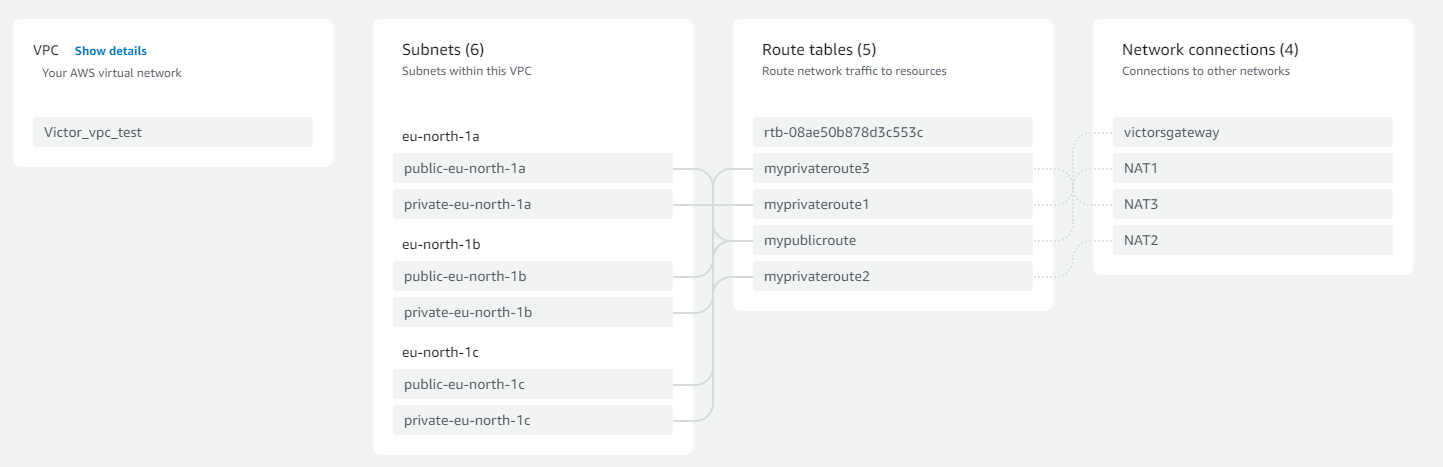
\includegraphics[scale=0.48]{graphics/aws_network.png}
\caption{\label{fig:aws_network} globaal overzicht van het netwerk}
\end{figure}

\begin{figure}[H]
  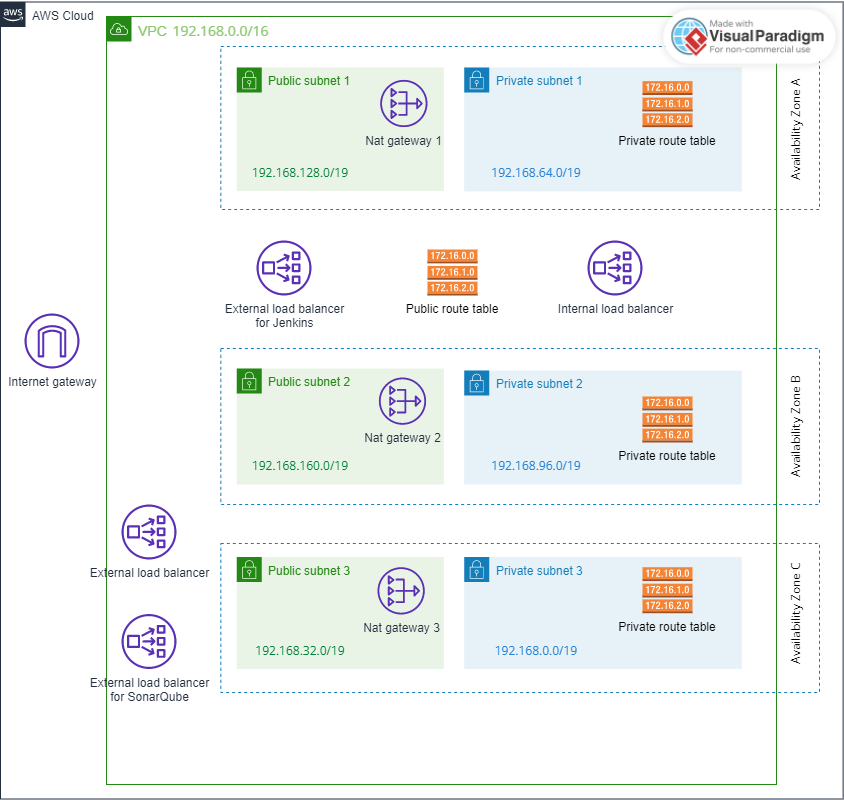
\includegraphics[scale=0.45]{graphics/network.png}
\caption{\label{fig:aws_networkfigure} het netwerk waarvan de POC opstelling gebruik maakt}
\end{figure}

\paragraph{\IfLanguageName{dutch}{Bouwen van het netwerk en de security groups met terraform}
{Building the network and the security groups using terraform}}
\label{sec:Bouwen van het netwerk en de security groups met terraform}

Om een omgeving in terraform op te stellen die hergebruikt kan worden, wordt bij elke component van het netwerk zoveel mogelijk met parameters gewerkt. De parameters worden ingesteld in het terraform tfvars bestand. Elke componente wordt ook waar mogelijk voorzien van een eigen module die ingeladen wordt in het main terraform bestand.
\newline

De VPC wordt op onderstaande manier opgebouwd. De id van de vpc die aangemaakt wordt, wordt gebruikt om andere componenten in het netwerk te configureren en wordt dus als een output voorzien binnen deze module.
\newline

\begin{lstlisting}[language=terraform]
  # Bouwen van een aws vpc component
  resource "aws_vpc" "main" {
  
    # Instellen van de vpc cidr block
    cidr_block = var.vpc_cidr
  
    # Instellen van de vpc naam
    tags = var.vpc_name
  
    # aanzetten van bepaalde dns instellingen die nodig zijn voor deze vpc
    enable_dns_hostnames = true
    enable_dns_support = true
  
  }
\end{lstlisting}

\vspace{0.5cm}
De subnets worden voorzien van ingress and egress regels zodat het netwerkverkeer gecontroleerd kan worden van en naar de verschillende netwerkcomponenten. Om deze regels te kunnen configureren moeten er eerst security groups aangemaakt worden. Deze security groups worden vervolgens gelinkt met toepasselijke regels. De security groups worden op deze manier geconfigureerd. Deze componten in de opstelling zijn afhankelijk van de VPC en gebruiken de output van de VPC module om correct ingesteld te worden.
\newline

\begin{lstlisting}[language=terraform]
  # Resource block die gebruikt wordt om een security group aan te maken
  resource "aws_security_group" "group1" { 
  
    # Instellen van de security group naam
    name   = var.aws_security_group
  
    # Instellen van de vpc id
    vpc_id = var.vpc_id 
  
    # Instellen van de security group tags
    tags = var.aws_security_group_name
  }
\end{lstlisting}

\vspace{0.5cm}
De verschillende ingress and egress regels worden geconfigureerd aan de hand van volgende terraform code. Afhankelijk van het soort regel worden enkele elementen toegevoegd bij de security group. Sommige regels worden niet geconfigureerd voor een bepaalde cidr, maar eerder voor een bepaalde security group. Daarnaast zijn sommige regels ook geconfigureerd om alle protcollen toe te laten. Welke instelling een regel krijgt hang af van hoe deze georienteerd staat, met andere woorden of het om een ingress of egress regel gaat. Bij deze modules wordt ook gebruik gemaakt van data sources en locals om alle parameters in te stellen.
\newline

De terraform configuratie voor een ingress rule met als bron een bepaalde security group ziet er zo uit.
\newline

\begin{lstlisting}[language=terraform]
  # Resource block die gebruikt wordt om een ingress rule in te stellen
  resource "aws_vpc_security_group_ingress_rule" "name" {
  
      # Instellen van het bereik (van poort ... tot poort ...)
      from_port = var.aws_security_group_from
      to_port = var.aws_security_group_to
  
      # Instellen van het protocol waarop deze security rule van toepassing is tcp/udp of -1 voor beide
      ip_protocol = var.aws_security_group_rule_protocol
  
      # Id van de security group die gebruikt zal worden als de source van het verkeer
      referenced_security_group_id = data.aws_security_group.source.id
  
      # Id van de security group zodat deze rule aan deze group gekoppeld kan worden
      security_group_id = data.aws_security_group.name.id
    
  }
\end{lstlisting}

\vspace{0.5cm}
De terraform configuratie voor een ingress rule met als bron een cidr wordt op deze manier geconfigureerd.
\newline

\begin{lstlisting}[language=terraform]
  # Resource block die gebruikt wordt om een ingress rule in te stellen
  resource "aws_vpc_security_group_ingress_rule" "name" {
  
      # de cidr die gebruikt zal worden als de source van het verkeer
      cidr_ipv4 = local.cidr_ipv4
  
      # Instellen van het bereik (van poort ... tot poort ...)
      from_port = var.aws_security_group_from
      to_port = var.aws_security_group_to
  
      # Instellen van het protocol waarop deze security rule van toepassing is tcp/udp of -1 voor beide
      ip_protocol = var.aws_security_group_rule_protocol
  
      # Id van de security group zodat deze rule aan deze group gekoppeld kan worden
      security_group_id = data.aws_security_group.name.id
    
  }
\end{lstlisting}

\vspace{0.5cm}
De terraform configuratie voor een egress rule met als bestemming een cidr ziet er zo uit.
\newline

\begin{lstlisting}[language=terraform]  
  # Resource block die gebruikt wordt om een ingress rule in te stellen
  resource "aws_vpc_security_group_egress_rule" "name" {
  
      # de cidr die gebruikt zal worden als de source van het verkeer
      cidr_ipv4 = local.cidr_ipv4
      
      # Instellen van het protocol waarop deze security rule van toepassing is tcp/udp of -1 voor beide
      ip_protocol = var.aws_security_group_rule_protocol
  
      # Id van de security group zodat deze rule aan deze group gekoppeld kan worden
      security_group_id = data.aws_security_group.name.id
    
  }
\end{lstlisting}

\vspace{0.5cm}
De VPC is gelinkt met alle subnets. Bij deze opstelling worden private en publieke subnets voorzien. Deze subnets zijn verspreid over meerder availability zones op die manier is er extra redundantie. De id's van de aangemaakte subnets worden gebruikt voor het maken van de servers en de cluster.
\newline

De configuratie om een private subnet in te stellen kan hieronder teruggevonden worden. Bij de configuratie van een publiek subnet wordt de parameter "map public ip on launch toegevoegd".
\newline
\begin{lstlisting}[language=terraform]  
  # Resource block die gebruikt wordt om een private subnet in te stellen
  resource "aws_subnet" "private_subnet" {
  
    # Instellen van de VPC id
    vpc_id     = var.vpc_id
  
    # Instellen van de cidr
    cidr_block = var.private_subnet_cidr
  
    # Instellen van de naam en andere tags
    tags       = var.private_subnet_tags
  
    # Instellen van de AWS availability zone
    availability_zone = var.private_subnet_availability_zone
  } 
\end{lstlisting}

\vspace{0.5cm}
De meeste basis componenten van het netwerk zijn op dit moment geconfigureerd, maar de toegang naar het internet ontbreekt nog, de gateways. De publieke subnets worden gelinkt aan één internet gateway en de private worden elk voorzien van een nat gateway. Op die manier kunnen instanties uit de verschillende subnets aan het internet indien dit een vereiste zou zijn.
\newline

De internet gateway wordt op deze manier geconfigureerd. De id van deze resource wordt gebruikt voor het configureren van de route tabellen.
\newline

\begin{lstlisting}[language=terraform]  
  # Resource block die gebruikt wordt om een internet gateway in te stellen
  resource "aws_internet_gateway" "name" {
  
      # Instellen van de VPC id
      vpc_id = var.vpc_id
  
      # Instellen van de internet gateway naam
      tags = var.aws_internet_gateway_name
  
    
  }
\end{lstlisting}

\vspace{0.5cm}
In een nat gateway worden de private ip-adressen vertaald naar publieke, daarom moeten er eerst nog elastic ip-adressen geconfigureerd worden in AWS. Elastic ip-adressen zorgen ervoor dat de nat gateways een publiek adres krijgen. De elastic ip-adressen worden op deze manier geconfigureerd.
\newline

\begin{lstlisting}[language=terraform]  
  # Resource block die gebruikt wordt om een elastic ip-adres in te stellen
  resource "aws_eip" "nat1" {
  
      # Instellen van de elastic ip adres naam
      tags = var.aws_eip_name 
  }
\end{lstlisting}

\vspace{0.5cm}
Om de nat gateways te configureren wordt deze terraform configuratie gebruikt. De output van deze component wordt opnieuw gebruikt bij het bouwen van de verschillende route tabellen.
\newline

\begin{lstlisting}[language=terraform]  
  # Resource block die gebruikt wordt om een nat gateway in te stellen
  resource "aws_nat_gateway" "example" {
  
    # Instellen van het elastic ip adres dat gekoppelt wordt aan deze resource
    allocation_id = var.aws_eip_id
  
    # Instellen van het publieke subnet dat gekoppelt wordt aan deze resource
    subnet_id     = var.public_subnet_id
  
    # Instellen van de nat gateway naam
    tags = var.aws_nat_gateway_name
  }
\end{lstlisting}

\vspace{0.5cm}
De laatste stap om het netwerk werkende te krijgen is het toevoegen van de routes. Alle componenten zijn ondertussen al opgebouwd, maar er is nog geen route tabel gebouwd die ervoor zorgt dat de resource het internet kunnen gebruiken. Om deze laatste stap van het netwerk correct te configureren wordt gebruik gemaakt van de "AWS route table" resource. 
\newline

Om een private route tabel te configureren wordt volgende code blok gebruikt. Bij een publieke route tabel wordt gebruik gemaakt van de nat gateway id in de plaats van de internet gateway id.
\newline

\begin{lstlisting}[language=terraform]  
  # Resource block die gebruikt wordt om een nat gateway in te stellen
  resource "aws_route_table" "route_table_private" {
  
      # Instellen van de VPC id
      vpc_id = var.aws_vpc_id
  
      # Instellen van de route
      route {
  
          # Instellen van de cidr
          cidr_block = var.aws_route_table_private_cidr
  
          # Instellen van de gateway die gebruikt zal worden
          gateway_id = var.aws_nat_gateway_id
      }
  
      # Instellen van de route tabel naam
      tags = var.aws_route_table_private_name
    
  }
\end{lstlisting}

\vspace{0.5cm}
De route tabellen moeten uiteindelijk nog gelinkt worden aan de correcte subnets. Via volgende code wordt deze link op de juiste manier opgebouwd.

\begin{lstlisting}[language=terraform]  
  # Resource block die gebruikt wordt om een route tabel link in te stellen
  resource "aws_route_table_association" "route_association_public" {
      
      # Instellen van het correcte subnet
      subnet_id = var.aws_subnet_public_id
  
      # Instellen van de route tabel die gebruikt zal worden
      route_table_id = var.aws_route_table_public_id
  }
  
\end{lstlisting}

% \paragraph{\IfLanguageName{dutch}{Infrastructuur overzicht}
% {Overview of the infrastructure}}
% \label{sec:Infrastructuur overzicht}

De infrastructuur wordt opgebouwd door gebruik te maken van terraform. In deze opstelling worden enkele servers voorzien. De jenkins server is verantwoordelijk voor alle bouwopdrachten. Deze server is het hart van de CD pipeline. De bouwopdrachten worden niet rechstreeks uitgevoerd op deze server, deze server stuurt een AWS autoscaling groep aan die nieuwe ec2 instances toevoegt wanneer nieuwe builds worden aangevraagd. Door gebruik te maken van een autoscaling groep is het mogelijk om deze instances ook af te breken wanneer deze niet meer nodig zijn. 
\newline

De bouwopdrachten worden dus uitgevoerd op aparte ec2 instances, genaamd jenkins runners. De jenkins runners en de jenkins master server maken beide gebruik van een baked image op die manier is er geen nood aan extra scripts wanneer de instance  opgestart wordt. Deze manier van werken laat ook toe om verschillende soorten jenkins runners te bouwen voor verschillende soorten pipelines. De configuratie van de jenkins server wordt voorzien aan de hand van een "jenkins as code". Deze configuratie file is opgeslagen in een aparte S3 bucket en wordt ingeladen bij het opstarten van de jenkins server.
\newline

Deze jenkins server is niet direct verbonden met het internet er is een loadbalancer voorzien om toegang te krijgen tot de login pagina. Deze server is ook enkel beschikbaar in een private subnet. Er wordt gebruik gemaakt van een nat gateway om internet te voorzien en via een bastion server is er een mogelijkheid om naar deze machine te sshen.
\newline

Verder is op deze server ook een sonarqube container aanwezig die sonarqube voorziet. Ook sonarqube is toegankelijk via een loadbalancer. De jenkinsserver beschikt daarnaast over enkele software die nodig is om correct te functioneren.
\newline


% \begin{figure}[H]
%   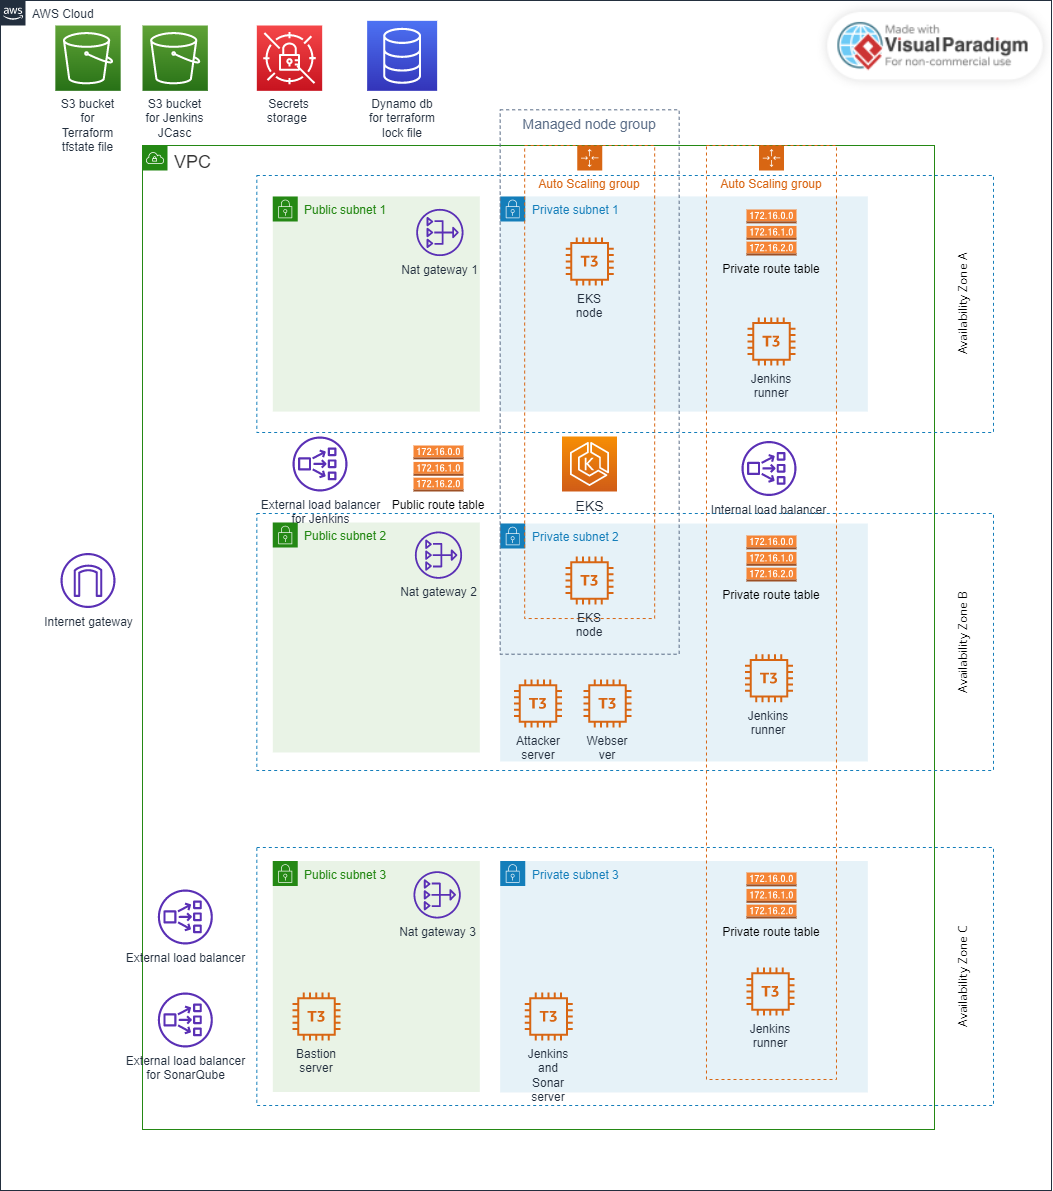
\includegraphics[scale=0.50]{graphics/infrastructuur.png}
% \caption{\label{fig:aws_infrastructuur} De infrastructuur waar de POC gebruik van maakt}
% \end{figure}

% \paragraph{\IfLanguageName{dutch}{Bouwen van de infrastructuur met terraform}
% {Building the infrastructure with terraform}}
% \label{sec:Bouwen van de infrastructuur met terraform}





























































\subsubsection{\IfLanguageName{dutch}{Post deployment}
{Post deployment}}
\label{sec:Post deployment}

\subsection{\IfLanguageName{dutch}{De CI/CD pipeline opzetten}
{Building the CI/CD pipeline}}
\label{sec:Bouwen van de CI/CD pipeline}

\subsubsection{\IfLanguageName{dutch}{Bouwen van de CI pipeline}
{Building the CI pipeline}}
\label{sec:Bouwen van de CI pipeline}

\subsubsection{\IfLanguageName{dutch}{Bouwen van de CD pipeline}
{Building the CI/CD pipeline}}
\label{sec:Bouwen van de CD pipeline}

\section{\IfLanguageName{dutch}{Aanvallen op de POC omgeving}
{Attacks on the POC environment}}
\label{sec:Aanvallen op de POC omgeving}

\subsection{\IfLanguageName{dutch}{Aanval 1}
{Aanval 1}}
\label{sec:Aanval 1}

\subsubsection{\IfLanguageName{dutch}{Aanval scenario}
{Attack scenario}}
\label{sec:Aanval scenario}

\subsubsection{\IfLanguageName{dutch}{Impact}
{Impact}}
\label{sec:Impact}

\subsubsection{\IfLanguageName{dutch}{Aanbevelingen}
{Recommendations}}
\label{sec:Aanbevelingen}

\subsection{\IfLanguageName{dutch}{Aanval 2}
{Aanval 2}}
\label{sec:Aanval 2}

\subsubsection{\IfLanguageName{dutch}{Aanval scenario}
{Attack scenario}}
\label{sec:Aanval scenario}

\subsubsection{\IfLanguageName{dutch}{Impact}
{Impact}}
\label{sec:Impact}

\subsubsection{\IfLanguageName{dutch}{Aanbevelingen}
{Recommendations}}
\label{sec:Aanbevelingen}

\subsection{\IfLanguageName{dutch}{Aanval 3}
{Aanval 3}}
\label{sec:Aanval 3}

\subsubsection{\IfLanguageName{dutch}{Aanval scenario}
{Attack scenario}}
\label{sec:Aanval scenario}

\subsubsection{\IfLanguageName{dutch}{Impact}
{Impact}}
\label{sec:Impact}

\subsubsection{\IfLanguageName{dutch}{Aanbevelingen}
{Recommendations}}
\label{sec:Aanbevelingen}

\subsection{\IfLanguageName{dutch}{Aanval 4}
{Aanval 4}}
\label{sec:Aanval 4}

\subsubsection{\IfLanguageName{dutch}{Aanval scenario}
{Attack scenario}}
\label{sec:Aanval scenario}

\subsubsection{\IfLanguageName{dutch}{Impact}
{Impact}}
\label{sec:Impact}

% werken met kaders mss

\subsubsection{\IfLanguageName{dutch}{Aanbevelingen}
{Recommendations}}
\label{sec:Aanbevelingen}


\begin{itemize}
  \item De AWS rollen die gebruikt worden om toegang te verlenen tot de verschillende AWS services, zijn enkel voorzien van de nodige permissies.
  \item Er wordt gebruik gemaakt van een bastionserver om toegang te verlenen tot de verschillende servers.
  \item De omgeving bestaat uit publieke en prive subnetten zodat de belangrijkste instantie niet zomaar toegankelijk zijn vanaf het internet.
  \item Er wordt zoveel mogelijk gebruik gemaakt van ssh waar dit mogelijk is.
  \item Wanneer er gebruik wordt gemaakt van secrets zijn deze ogeslagen in de secret kluis van AWS.
\end{itemize}

% Voeg hier je eigen hoofdstukken toe die de ``corpus'' van je bachelorproef
% vormen. De structuur en titels hangen af van je eigen onderzoek. Je kan bv.
% elke fase in je onderzoek in een apart hoofdstuk bespreken.

%\input{...}
%\input{...}
%...

%%=============================================================================
%% Conclusie
%%=============================================================================

\chapter{Conclusie}%
\label{ch:conclusie}

% TODO: Trek een duidelijke conclusie, in de vorm van een antwoord op de
% onderzoeksvra(a)g(en). Wat was jouw bijdrage aan het onderzoeksdomein en
% hoe biedt dit meerwaarde aan het vakgebied/doelgroep? 
% Reflecteer kritisch over het resultaat. In Engelse teksten wordt deze sectie
% ``Discussion'' genoemd. Had je deze uitkomst verwacht? Zijn er zaken die nog
% niet duidelijk zijn?
% Heeft het onderzoek geleid tot nieuwe vragen die uitnodigen tot verder 
%onderzoek?

\lipsum[76-80]



%---------- Bijlagen -----------------------------------------------------------

\appendix

\chapter{Onderzoeksvoorstel}

Het onderwerp van deze bachelorproef is gebaseerd op een onderzoeksvoorstel dat vooraf werd beoordeeld door de promotor. Dat voorstel is opgenomen in deze bijlage.

%% TODO: 
%\section*{Samenvatting}

% Kopieer en plak hier de samenvatting (abstract) van je onderzoeksvoorstel.

% Verwijzing naar het bestand met de inhoud van het onderzoeksvoorstel
%---------- Inleiding ---------------------------------------------------------

\section{Introductie}%
\label{sec:introductie}

De nood aan het sneller opleveren van betere code neemt elk jaar toe. \footnote{https://brfplus.co.uk/the-increasing-demand-for-low-code-skills/} Om die reden zijn de eerste Continuous integration/Continous delivery (CI/CD) en deploy pipelines ontwikkeld. Software updates kwamen voorheen minder frequent voor. Het snel uitbrengen van updates werd niet ondersteund door de hardware- en programmeertalen die beschikbaar waren in de jaren 60 \autocite{Jiang2009}. Het kon jaren duren vooraleer een nieuwe update uitgebracht werd. Door de opkomst van Agile methodes in de sofware industrie is het mogelijk geworden om sneller updates uit te brengen. 

Met behulp van CI/CD pipelines liggen de huidige release cycli veel dichter bij elkaar. \footnote{https://www.jetbrains.com/teamcity/ci-cd-guide/benefits-of-ci-cd/} Software wordt verwerkt in kleine iteraties waardoor er veel minder kans is op langdurige bugs en of problemen wanneer de deploy stap bereikt wordt. Ook de testfase is veel beter geïntegreerd dankzij deze aanpak. In de verschillende fasen van een CI/CD pipeline wordt er gebruikt gemaakt van secrets. Secrets worden gebruikt voor de beveiliging van allerhande services zoals Docker Hub, GitHub, Kubernetes, Web APIs. De manier waarop omgegaan wordt met deze gevoelige informatie, kan in vraag gesteld worden. \footnote{https://maia.crimew.gay/posts/how-to-hack-an-airline/} Daarom is het belangrijk dat de risico’s in kaart worden gebracht en dat er onderzoek wordt uitgevoerd naar eventuele “best practices” of alternatieven om op een veilige manier om te gaan met secrets. Ieder devops team dat gebruik maakt van een Jenkins pipeline is kwetsbaar en heeft er baat bij om te weten te komen hoe zij dit risico zo laag mogelijk kunnen houden. Het is belangrijk dat zij inzien welke alternatieven mogelijks gebruikt kunnen worden om de integriteit, confidentialiteit en beschikbaarheid van hun pipeline te garanderen.  

Binnen dit onderzoek zal gebruik gemaakt worden van de Jenkins software voor het opzetten van een CI/CD server. Via een proof of concept wordt nagegaan voor welke aanvallen deze server het kwetsbaarst is en hoe deze gevoelige informatie gestolen kan worden. Allereerst zal er onderzocht worden op welke manier er wordt omgegaan met secrets binnen de CI/CD server. Daarna is het de bedoeling de verschillende soorten aanvallen die mogelijk zijn op deze CI/CD server in kaart te brengen. Vervolgens wordt onderzocht hoe deze vertrouwelijke informatie geëxtraheerd kan worden via deze aanvallen. Via een testomgeving worden deze aanvallen gedocumenteerd. Uiteindelijk wordt op zoek gegaan naar alternatieve methodes om secrets op een veilige manier te transporteren doorheen het CI/CD proces. Aan de hand van een overzicht worden de “best practices” en eventuele alternatieve methodes in detail beschreven.

\section{State-of-the-art}%
\label{sec:state-of-the-art}

Om na te gaan hoe veilig het is om secrets te gebruiken in een CI/CD pipeline, moet er eerst onderzocht worden hoe deze gevoelige informatie gebruikt worden in deze omgeving. Secrets kunnen opgeslagen worden in omgevingsvariabelen en kunnen gebruikt worden als “secrets as code”. Dit is echter niet de meest veilige manier. \textcite{Pecka2022} tonen aan in hun paper wanneer toegang verkregen wordt tot de CI/CD pipeline, het zeer eenvoudig is om geheime informatie op te halen voor bijvoorbeeld een Kubernetes cluster. Het is dan ook niet meer moeilijk om binnen te treden in de achterliggende infrastructuur. \textcite{Gil} beschrijven hoe het mogelijk is omgevingsvariabelen uit te lezen via een “Poisened Pipeline Execution” aanval. Doordat variabelen ingesteld worden op “configuration as code” niveau, is de kans op dergelijke aanvallen groot. Het is belangrijk dat wanneer secrets op deze manier worden opgeslagen, dit van tijdelijk aard is en dat er op zoek wordt gegaan naar alternatieven zodat deze gevoelige informatie beter beheerd kan worden. Het beheren van vertrouwelijke informatie aan de hand van omgevingsvariabelen en configuratie bestanden blijft een veel gebruikte methode in de praktijk. Er is onvoldoende hygiëne wanneer er wordt omgegaan met secrets zoals blijkt uit de tekst van \autocite{Gil}. 

Wanneer secrets gebruikt worden in een devops omgeving is het van belang dat deze op een veilige manier bewaard worden en dat deze vertrouwelijke informatie enkel toegankelijk is voor geautoriseerde personen. Er bestaan verschillende manieren om confidentialiteit, integriteit en beschikbaarheid te garanderen. Door gebruik te maken van encryptie is het mogelijk een extra beschermingslaag te voorzien. \textcite{Kuzminykh2020} beschrijven in hun studie welke aspecten het belangrijkste zijn wanneer er gebruik wordt gemaakt van een managementsysteem om secrets op te slaan.  Eén van de belangrijkste aspecten voor een kleine tot middelgrote organisatie, is het voorzien van een beveiligde communicatie waarbij rekening gehouden wordt met encryptie. \autocite{AaronHaymore} beschrijven waarom het gebruik van deze managementsystemen niet de enigste instrumenten mogen zijn wanneer een devops omgeving beveiligd wordt. De S3 Bucket is een zeer veel gebruikte service om credentials en andere geheime informatie op te slaan binnen een Amazon cloud omgeving. Wanneer dit systeem niet correct geconfigureerd is, is het zeer eenvoudig toegang te verkrijgen tot de achterliggende servers en bijgevolg toegang tot het CI/CD proces. Op het evenement Black Hat USA 2022 \autocite{Gazdag} werd er toegelicht waarom het van cruciaal belang is dat er op een correcte manier omgegaan wordt met geheime informatie. Bij hun aanvallen op CI/CD pipelines, kwamen zij vaak het eerst in aanraking met secrets en daardoor was het eenvoudig toegang te verkrijgen tot de achterliggende software. 

Het is belangrijk dat er bepaalde controleorganen beschikbaar zijn die gebruikt kunnen worden als toegangscontrole wanneer secrets nodig zijn, bijvoorbeeld door het toevoegen van multifactorauthenticatie of een toegangscontrole beleid. Een tweede beschermingslaag boven op de geëncrypteerde connectie is van belang en heeft alleen maar voordelen. Incorrecte implementatie van toegangscontrole zorgt ervoor dat het CI/CD platform niet veilig is en niet vertrouwd kan worden. Uit een onderzoek van USENIX \autocite{Koishybayev2022} blijkt dat toegangscontroles voor secrets zeker nog niet bij alle CI/CD frameworks correct geïmplementeerd zijn.


% Voor literatuurverwijzingen zijn er twee belangrijke commando's:
% \autocite{KEY} => (Auteur, jaartal) Gebruik dit als de naam van de auteur
%   geen onderdeel is van de zin.
% \textcite{KEY} => Auteur (jaartal)  Gebruik dit als de auteursnaam wel een
%   functie heeft in de zin (bv. ``Uit onderzoek door Doll & Hill (1954) bleek
%   ...'')


%---------- Methodologie ------------------------------------------------------
\section{Methodologie}%
\label{sec:methodologie}

De eerste weken zullen gebruikt worden om een literatuurstudie op te stellen. Op die manier kan de context waarin de onderzoeksvraag verweven zit beter geschetst worden. Dit onderzoek zal gericht zijn op hoe secrets gebruikt worden in deze omgeving. 

In de volgende fase wordt er op zoek gegaan naar aanvallen die mogelijk zijn op een CI/CD pipeline. Via de informatie die verkregen werd in de vorige fase, is het mogelijk gerichter te onderzoeken welke aanvallen het meest betrekking hebben tot de Jenkins pipeline.  Wanneer een duidelijk overzicht verkregen wordt van de meest nuttige aanvallen, is het de bedoeling deze aanvallen te testen aan de hand van een testomgeving. Via de CI/CD Goat \footnote{https://github.com/cider-security-research/cicd-goat} is het mogelijk vertrouwd te geraken met de verschillende aanvallen. Deze kwetsbare CI/CD omgeving is een hulpinstrument waarop verschillende testen uitgevoerd kunnen worden. Bij de testen zal er onderzocht worden welke rol secrets spelen in het aanvalsproces.  

De derde fase start met een studie naar alternatieve methodes om  een Jenkins pipeline te beveiligen. Doordat er een bepaalde kennis is over de aanvallen en het Jenkins platform zelf is het mogelijk een Proof of concept (POC) op te stellen. Via deze POC wordt een overzicht verkregen welke beveiligingsmethodes het meest effectief zijn.

Uiteindelijk wordt een toelichting en advies gegeven waarin de “best practices” en alternatieve methodes omschreven worden. Daarnaast zal er bij deze finale fase een handleiding worden opgesteld om een Jenkins pipeline te beveiligen.


%---------- Verwachte resultaten ----------------------------------------------
\section{Verwacht resultaat, conclusie}%
\label{sec:verwachte_resultaten}

Er bestaan tal van mogelijkheden om een CI/CD pipeline aan te vallen waardoor deze omgeving redelijk snel aangetast kan worden. Een threat actor die toegang heeft tot de pipeline kan de achterliggende infrastructuur binnendringen wanneer niet op een correcte manier gebruik wordt gemaakt van secrets. Gelukkig door het toevoegen van nieuwe aanvullingen, zoals software om secrets te beheren en extra authenticatie mogelijkheden, kunnen secrets met meer vertrouwen gebruikt worden. Het blijft wel belangrijk om de basisprincipes van security steeds in acht te nemen. Hoe veilig een CI/CD omgeving uiteindelijk is, hangt af van zijn zwakste schakel. Deze zwakste schakel ontstaat nog steeds meestal door een menselijke fout. Het is belangrijk dat het personeel dat gebruik maakt van de CI/CD omgeving goed opgeleid is en dat dit personeel slechts toegang heeft volgens het principe van “least privilege”. 

%%---------- Andere bijlagen --------------------------------------------------
% TODO: Voeg hier eventuele andere bijlagen toe. Bv. als je deze BP voor de
% tweede keer indient, een overzicht van de verbeteringen t.o.v. het origineel.
%\input{...}
%%=============================================================================
%% Bijlagen
%%=============================================================================

\chapter{\IfLanguageName{dutch}{Bijlagen}{Appendix}}%
\label{ch:Bijlagen}

\section{\IfLanguageName{dutch}{Variabelen, inputs, outputs, data sources en locals voor het bouwen van het netwerk en de security groups met terraform}
{Variables to build the network and the security groups using terraform}}
\label{sec:Variabelen voor het bouwen van het netwerk en de security groups met terraform}

\subsection{\IfLanguageName{dutch}{VPC}
{VPC}}
\label{sec:VPC}

\subsubsection{\IfLanguageName{dutch}{Input}
{Input}}
\label{sec:Input}

\begin{lstlisting}[language=terraform]
    variable "vpc_cidr" {
        type = string
        default = "192.168.0.0/16"
        
      }
      
      variable "vpc_name" {
          type = map(any)
          default = {
              Name = "My_vpc"
          }
        
      }
      
      variable "vpc_enable_dns_hostnames" {
        type = bool
        default = true
      
        
      }
      
      variable "vpc_enable_dns_support" {
        type = bool
        default = true
      } 
\end{lstlisting}

\subsubsection{\IfLanguageName{dutch}{Output}
{Output}}
\label{sec:Output}

\begin{lstlisting}[language=terraform]
    output "vpc_id" {
        value = aws_vpc.main.id
    }   
\end{lstlisting}

\subsubsection{\IfLanguageName{dutch}{Variables}
{Variables}}
\label{sec:Variables}

\begin{lstlisting}[language=terraform]
  vpc_cidr = "192.168.0.0/16"

  vpc_name = {Name = "Victor_vpc_test"}
  
  vpc_enable_dns_hostnames = true
  
  vpc_enable_dns_support = true
\end{lstlisting}

\subsection{\IfLanguageName{dutch}{VPC security group}
{VPC security group}}
\label{sec:VPC security group}

\subsubsection{\IfLanguageName{dutch}{Input}
{Input}}
\label{sec:Input}

\begin{lstlisting}[language=terraform]
    variable "aws_security_group" {
        type = string
        default = "testgroup"
    }
    
    variable "aws_security_group_name" {
        type = map(any)
        default = {Name = "mysecuritygroup"}
      
    }
    
    variable "vpc_id" {
        type = string
        default = ""
      
    }
\end{lstlisting}

\subsubsection{\IfLanguageName{dutch}{Variables}
{Variables}}
\label{sec:Variables}

\begin{lstlisting}[language=terraform]
  security_group_config = {
    group1 = {
        aws_security_group = "security_group_bastion"
        aws_security_group_name = {Name="securitygroup_bastion"}
    },  
    group2 = {
        aws_security_group = "security_group_jenkins"
        aws_security_group_name = {Name="securitygroup_jenkins"}
    }

    group3 = {
        aws_security_group = "security_group_lb"
        aws_security_group_name = {Name="securitygroup_lb"}
    }
    group4 = {
        aws_security_group = "security_group_jenkins_slaves"
        aws_security_group_name = {Name="securitygroup_jenkins_slaves"}
    }
}
\end{lstlisting}

\subsection{\IfLanguageName{dutch}{VPC security group rules}
{VPC security group rules}}
\label{sec:VPC security group regels}

\subsubsection{\IfLanguageName{dutch}{Input}
{Input}}
\label{sec:Input}

\begin{lstlisting}[language=terraform]
    variable "aws_security_group" {
        type = string
        default = "testgroup"
    }
    
    variable "aws_security_group_from" {
      type = number
    }
    
    variable "aws_security_group_to" {
      type = number
    }
    
    variable "aws_security_group_rule_protocol" {
      type = string
    }
    
    variable "aws_security_group_cidr" {
        type = string
      
    }   
\end{lstlisting}

\subsubsection{\IfLanguageName{dutch}{Data source}
{Data source}}
\label{sec:Data source}

\begin{lstlisting}[language=terraform]
    # Data block om de security group id op te halen van de source
    data "aws_security_group" "source" {
    
        # Variabele die gebruikt wordt om deze id op te halen
        name = var.aws_security_group_source
      
    }
    
    # Data block om de security group id op te halen waar de rule aan gelinkt zal worden
    data "aws_security_group" "name" {
    
        # Variabele die gebruikt wordt om deze naam op te halen
        name = var.aws_security_group
      
    }
\end{lstlisting}

\subsubsection{\IfLanguageName{dutch}{locals}
{Locals}}
\label{sec:Locals}

\begin{lstlisting}[language=terraform]
    # Bepalen of de cidr variable leeg is of niet
    locals {
    
      # Gebruik maken van de length function om te bepalen of de security group cidr is leeg, indien leeg return a null object
      cidr_ipv4 = length(var.aws_security_group_cidr) > 0 ? var.aws_security_group_cidr : null
    }
    
\end{lstlisting}

\subsubsection{\IfLanguageName{dutch}{Variables}
{Variables}}
\label{sec:Variables}

\begin{lstlisting}[language=terraform]
  security_group_ingress_rules_config = {
    rule1 = {
        aws_security_group = "security_group_bastion"
        aws_security_group_from = 22
        aws_security_group_to = 22
        aws_security_group_source = ""
        aws_security_group_rule_protocol = "tcp"
        aws_security_group_cidr = "0.0.0.0/0"

    },
    rule2 = {
        aws_security_group = "security_group_jenkins"
        aws_security_group_from = 8080
        aws_security_group_to = 8080
        aws_security_group_source = ""
        aws_security_group_rule_protocol = "tcp"
        aws_security_group_cidr = "0.0.0.0/0"
    },
    rule3 = {
        aws_security_group = "security_group_lb"
        aws_security_group_from = 80
        aws_security_group_to = 80
        aws_security_group_source = ""
        aws_security_group_rule_protocol = "tcp"
        aws_security_group_cidr = "0.0.0.0/0"
    }
    rule4 = {
        aws_security_group = "security_group_jenkins"
        aws_security_group_from = 9000
        aws_security_group_to = 9000
        aws_security_group_source = ""
        aws_security_group_rule_protocol = "tcp"
        aws_security_group_cidr = "0.0.0.0/0"
    },

}

security_group_ingress_rules_config_nocidr = {
    rule1 = {
        aws_security_group = "security_group_jenkins"
        aws_security_group_from = 22
        aws_security_group_to = 22
        aws_security_group_source = "security_group_bastion"
        aws_security_group_rule_protocol = "tcp"

    },
    rule2 = {
        aws_security_group = "security_group_jenkins"
        aws_security_group_from = 8080
        aws_security_group_to = 8080
        aws_security_group_source = "security_group_lb"
        aws_security_group_rule_protocol = "tcp"
    }
    rule3 = {
        aws_security_group = "security_group_jenkins"
        aws_security_group_from = 9000
        aws_security_group_to = 9000
        aws_security_group_source = "security_group_lb"
        aws_security_group_rule_protocol = "tcp"
    },
    rule4 = {
        aws_security_group = "security_group_jenkins_slaves"
        aws_security_group_from = 22
        aws_security_group_to = 22
        aws_security_group_source = "security_group_jenkins"
        aws_security_group_rule_protocol = "tcp"
    },

}

security_group_egress_rules_config = {
    rule1 = {
        aws_security_group = "security_group_bastion"
        aws_security_group_source = ""
        aws_security_group_rule_protocol = "-1"
        aws_security_group_cidr = "0.0.0.0/0"

    },
    rule2 = {
        aws_security_group = "security_group_jenkins"
        aws_security_group_source = ""
        aws_security_group_rule_protocol = "-1"
        aws_security_group_cidr = "0.0.0.0/0"
    },
    rule3 = {
        aws_security_group = "security_group_lb"
        aws_security_group_source = ""
        aws_security_group_rule_protocol = "-1"
        aws_security_group_cidr = "0.0.0.0/0"
    },
    rule4 = {
        aws_security_group = "security_group_jenkins_slaves"
        aws_security_group_source = ""
        aws_security_group_rule_protocol = "-1"
        aws_security_group_cidr = "0.0.0.0/0"
    }

}
\end{lstlisting}

\subsection{\IfLanguageName{dutch}{Internet gateway}
{Internet gateway}}
\label{sec:Internet gateway}

\subsubsection{\IfLanguageName{dutch}{Input}
{Input}}
\label{sec:Input}

\begin{lstlisting}[language=terraform]
    variable "vpc_id" {
        type = string
        default = "myvpcid"
    
    }
    
    variable "aws_internet_gateway_name" {
        type = map(any)
        default = {
          "Name" = "mygateway" 
        }
    }
\end{lstlisting}

\subsubsection{\IfLanguageName{dutch}{Output}
{Output}}
\label{sec:Output}

\begin{lstlisting}[language=terraform]
    output "aws_internet_gateway_id" {
        value = aws_internet_gateway.name.id
      
    }
\end{lstlisting}

\subsubsection{\IfLanguageName{dutch}{Variables}
{Variables}}
\label{sec:Variables}

\begin{lstlisting}[language=terraform]
    aws_internet_gateway_name = {Name = "victorsgateway"}     
\end{lstlisting}

\subsection{\IfLanguageName{dutch}{Private en publieke subnets, nat gateways, AWS elastic ip-adressen en private route tabellen}
{Private en public subnets, nat gateways and AWS elastic ip-addresses and private routing tables}}
\label{sec:Private en publieke subnets, nat gateways and AWS elastic ip-adressen en private route tabellen}

\subsubsection{\IfLanguageName{dutch}{Input}
{Input}}
\label{sec:Input}

\begin{lstlisting}[language=terraform]
    variable "vpc_id" {
        type = string
        default = "myvpcid"
    
    }
    
    variable "public_subnet_cidr" {
        type = string
        default = "192.168.0.0/18"
      
    }
    
    variable "public_subnet_tags" {
        type = map(any)
        default = {
            Name = "my_subnet"
            "kubernetes.io/cluster/eks" = "shared"
            "kubernetes.io/role/elb" = 1
            
        }
      
    }
    
    variable "public_subnet_availability_zone" {
        type = string
        default = "eu-north-1a"
      
    }
    
    variable "public_subnet_publicip_onlaunch" {
      type = bool
      default = true
      
    }

    variable "aws_eip_name" {
        type = map(any)
        default = {
        Name = "nat1" 
        }
    
    }

    variable "aws_nat_gateway_name" {
        type = map(any)
        default = {
          Name = "mynatgateway"
        }
    }
      
    variable "aws_eip_id" {
        type = string
        default = "test"
    }
      
    variable "public_subnet_id" {
        type = string 
        default = "test"
    }

    variable "aws_route_table_private_cidr" {
        type = string
        default = "0.0.0.0/0"
    }
    
    variable "aws_nat_gateway_id" {
        type = string
    }
    
    variable "aws_route_table_private_name" {
        type = map(any)
        default = {
            Name = "myprivateroute"
            }
    }

    variable "aws_subnet_private_id" {
        type = string
    }
    
    variable "aws_route_table_private_id" {
        type = string
    }   
\end{lstlisting}

\subsubsection{\IfLanguageName{dutch}{Output}
{Output}}
\label{sec:Output}

\begin{lstlisting}[language=terraform]
    output "private_subnet_id" {
        value = aws_subnet.private_subnet.id
    }

    output "public_subnet_id" {
        value = aws_subnet.public_subnet.id
    }

    output "aws_eip_id" {
        value = aws_eip.nat1.id
    }

    output "aws_nat_gateway_id" {
        value = aws_nat_gateway.example.id
    }

    output "aws_route_table_private_id" {
        value = aws_route_table.route_table_private.id
    }
\end{lstlisting}

\subsubsection{\IfLanguageName{dutch}{Variables}
{Variables}}
\label{sec:Variables}

\begin{lstlisting}[language=terraform]
    private_subnet_config = {
        subnet1 = {
    
            private_subnet_cidr = "192.168.64.0/19"
            private_subnet_tags = {"Name" = "private-eu-north-1a"
            "kubernetes.io/cluster/eks" = "shared"
            "kubernetes.io/role/internal-elb" = 1
            }
            private_subnet_availability_zone = "eu-north-1a"
    
            aws_eip_name = {Name="nat1"}
    
            aws_nat_gateway_name = {Name="NAT1"}
    
            aws_route_table_private_cidr = "0.0.0.0/0"
            aws_route_table_private_name = {Name="myprivateroute1"}
        }
    
        subnet2 = {
    
            private_subnet_cidr = "192.168.96.0/19"
            private_subnet_tags = {"Name" = "private-eu-north-1b"
            "kubernetes.io/cluster/eks" = "shared"
            "kubernetes.io/role/internal-elb" = 1
            }
            private_subnet_availability_zone = "eu-north-1b"
    
            aws_eip_name = {Name="nat2"}
    
            aws_nat_gateway_name = {Name="NAT2"}
    
            aws_route_table_private_cidr = "0.0.0.0/0"
            aws_route_table_private_name = {Name="myprivateroute2"}
        },
    
        subnet3 = {
            private_subnet_cidr = "192.168.0.0/19"
            private_subnet_tags = {"Name" = "private-eu-north-1c"
            }
            private_subnet_availability_zone = "eu-north-1c"
    
            aws_eip_name = {Name="nat3"}
    
            aws_nat_gateway_name = {Name="NAT3"}
    
            aws_route_table_private_cidr = "0.0.0.0/0"
            aws_route_table_private_name = {Name="myprivateroute3"}
    
        }  
    
    }
    
    public_subnet_config = {
        
        subnet1 = {
            public_subnet_cidr = "192.168.128.0/19"
            public_subnet_tags = {"Name" = "public-eu-north-1a"
            "kubernetes.io/cluster/eks" = "shared"
            "kubernetes.io/role/elb" = 1
            }
            public_subnet_availability_zone = "eu-north-1a"
            public_subnet_publicip_onlaunch = true
    
            
        },
    
        subnet2 = {
            public_subnet_cidr = "192.168.160.0/19"
            public_subnet_tags = {"Name" = "public-eu-north-1b"
            "kubernetes.io/cluster/eks" = "shared"
            "kubernetes.io/role/elb" = 1
            }
            public_subnet_availability_zone = "eu-north-1b"
            public_subnet_publicip_onlaunch = true
        },
    
        subnet3 = {
            public_subnet_cidr = "192.168.32.0/19"
            public_subnet_tags = {"Name" = "public-eu-north-1c"
            }
            public_subnet_availability_zone = "eu-north-1c"
            public_subnet_publicip_onlaunch = true
    
    
        } 
    
    }   
\end{lstlisting}

\subsection{\IfLanguageName{dutch}{Publieke route tabellen}
{Public routing tables}}
\label{sec:Publieke route tabellen}

\subsubsection{\IfLanguageName{dutch}{Input}
{Input}}
\label{sec:Input}

\begin{lstlisting}[language=terraform]
    variable "aws_vpc_id" {
        type = string
    }
    
    variable "aws_route_table_public_cidr" {
        type = string
        default = "0.0.0.0/0"
    }
    
    variable "aws_internet_gateway_id" {
        type = string
    }
    
    variable "aws_route_table_public_name" {
        type = map(any)
        default = {
            Name = "mypublicroute"
            }
    }

    variable "aws_subnet_public_id" {
        type = string
    }
    
    variable "aws_route_table_public_id" {
        type = string
    }    
\end{lstlisting}

\subsubsection{\IfLanguageName{dutch}{Output}
{Output}}
\label{sec:Output}

\begin{lstlisting}[language=terraform]
    output "aws_route_table_public_id" {
        value = aws_route_table.route_table_public.id
    }
\end{lstlisting}

\subsubsection{\IfLanguageName{dutch}{Variables}
{Variables}}
\label{sec:Variables}

\begin{lstlisting}[language=terraform]
    aws_route_table_public_cidr = "0.0.0.0/0"
    aws_route_table_public_name = {Name="mypublicroute"}
\end{lstlisting}

\subsection{\IfLanguageName{dutch}{Overzicht van de modules}
{Overview of the modules}}
\label{sec:Overzicht van de modules}

\begin{lstlisting}[language=terraform]
    module "aws_vpc" {
        source = "./modules/vpc"
        vpc_cidr = var.vpc_cidr
        vpc_name = var.vpc_name
        vpc_enable_dns_hostnames = var.vpc_enable_dns_hostnames
        vpc_enable_dns_support = var.vpc_enable_dns_support     
    }
    
    module "aws_security_groups" {
        source = "./modules/aws_security_group"
        depends_on = [
          module.aws_vpc
        ]
        for_each = var.security_group_config
    
        aws_security_group = each.value.aws_security_group
        aws_security_group_name = each.value.aws_security_group_name
        vpc_id = module.aws_vpc.vpc_id
      
    }
    
    module "aws_security_group_rule_ingress" {
      source = "./modules/aws_security_group_rule_ingress"
      depends_on = [
        module.aws_security_groups
      ]
      for_each = var.security_group_ingress_rules_config
    
      aws_security_group = each.value.aws_security_group
      aws_security_group_from = each.value.aws_security_group_from
      aws_security_group_rule_protocol = each.value.aws_security_group_rule_protocol
      aws_security_group_to = each.value.aws_security_group_to
      aws_security_group_cidr = each.value.aws_security_group_cidr
      
    }
    
    module "aws_security_group_rule_ingres_nocidr" {
      source = "./modules/aws_security_group_rule_ingress_nocidr"
      depends_on = [
        module.aws_security_groups
      ]
      for_each = var.security_group_ingress_rules_config_nocidr
    
      aws_security_group = each.value.aws_security_group
      aws_security_group_from = each.value.aws_security_group_from
      aws_security_group_source = each.value.aws_security_group_source
      aws_security_group_rule_protocol = each.value.aws_security_group_rule_protocol
      aws_security_group_to = each.value.aws_security_group_to
      
    }
    
    module "aws_security_group_rule_egress" {
      source = "./modules/aws_security_group_rule_egress"
      depends_on = [
        module.aws_security_groups
      ]
      for_each = var.security_group_egress_rules_config
    
      aws_security_group = each.value.aws_security_group
      aws_security_group_rule_protocol = each.value.aws_security_group_rule_protocol
      aws_security_group_cidr = each.value.aws_security_group_cidr
      
    }
    
    module "aws_internet_gateway" {
        source = "./modules/aws_internet_gateway"
        vpc_id = module.aws_vpc.vpc_id
        aws_internet_gateway_name = var.aws_internet_gateway_name
    }
    
    module "private_subnet" {
        source = "./modules/privateSubnet"
        vpc_id = module.aws_vpc.vpc_id
    
        for_each = var.private_subnet_config
    
        private_subnet_availability_zone = each.value.private_subnet_availability_zone
        private_subnet_cidr = each.value.private_subnet_cidr
        private_subnet_tags = each.value.private_subnet_tags
      
    }
    
    module "public_subnet" {
        source = "./modules/publicSubnet"
        vpc_id = module.aws_vpc.vpc_id
    
        for_each = var.public_subnet_config
    
        public_subnet_availability_zone = each.value.public_subnet_availability_zone
        public_subnet_cidr = each.value.public_subnet_cidr
        public_subnet_tags = each.value.public_subnet_tags
        public_subnet_publicip_onlaunch = each.value.public_subnet_publicip_onlaunch
      
    }
    
    module "aws_eip" {
        source = "./modules/aws_eip"
        depends_on = [
          module.aws_internet_gateway   
        ]
    
        for_each = var.private_subnet_config
    
        aws_eip_name = each.value.aws_eip_name
      
    }
    
    
    
    module "aws_nat_gateway" {
        source = "./modules/aws_nat_gateway"
        depends_on = [
          module.aws_eip, module.public_subnet
        ]
    
        for_each = var.private_subnet_config
    
        aws_eip_id = module.aws_eip[each.key].aws_eip_id
        public_subnet_id = module.public_subnet[each.key].public_subnet_id
        aws_nat_gateway_name = each.value.aws_nat_gateway_name
    
    }
    
    module "aws_route_table_private" {
        source = "./modules/aws_route_table_private"
        depends_on = [
          module.aws_nat_gateway
        ]
    
        for_each = var.private_subnet_config
    
        aws_nat_gateway_id = module.aws_nat_gateway[each.key].aws_nat_gateway_id
        aws_route_table_private_cidr = each.value.aws_route_table_private_cidr
        aws_route_table_private_name = each.value.aws_route_table_private_name
        aws_vpc_id = module.aws_vpc.vpc_id
      
    }
    
    module "aws_route_table_public" {
        source = "./modules/aws_route_table_public"
        depends_on = [
          module.aws_nat_gateway
        ]
    
        aws_internet_gateway_id = module.aws_internet_gateway.aws_internet_gateway_id
        aws_route_table_public_cidr = var.aws_route_table_public_cidr
        aws_route_table_public_name = var.aws_route_table_public_name
        aws_vpc_id = module.aws_vpc.vpc_id
    }
    
    
    
    module "aws_route_table_association_private" {
      source = "./modules/aws_route_table_association_private"
      depends_on = [
        module.aws_route_table_private
      ]
    
      for_each = var.private_subnet_config
    
      aws_route_table_private_id = module.aws_route_table_private[each.key].aws_route_table_private_id
      aws_subnet_private_id = module.private_subnet[each.key].private_subnet_id
    
    }
    
    module "aws_route_table_association_public" {
      source = "./modules/aws_route_table_association_public"
      depends_on = [
        module.aws_route_table_public
      ]
    
      for_each = var.public_subnet_config
    
      aws_route_table_public_id = module.aws_route_table_public.aws_route_table_public_id
      aws_subnet_public_id = module.public_subnet[each.key].public_subnet_id
      
    }
\end{lstlisting}





%%---------- Backmatter, referentielijst ---------------------------------------

\backmatter{}

\setlength\bibitemsep{2pt} %% Add Some space between the bibliograpy entries
\printbibliography[heading=bibintoc]

\end{document}
